% !TeX program = pdfLaTeX
\documentclass[12pt]{article}
\usepackage{amsmath}
\usepackage{graphicx,psfrag,epsf}
\usepackage{enumerate}
\usepackage{natbib}
\usepackage{textcomp}
\usepackage[hyphens]{url} % not crucial - just used below for the URL
\usepackage{hyperref}

%\pdfminorversion=4
% NOTE: To produce blinded version, replace "0" with "1" below.
\newcommand{\blind}{0}

% DON'T change margins - should be 1 inch all around.
\addtolength{\oddsidemargin}{-.5in}%
\addtolength{\evensidemargin}{-.5in}%
\addtolength{\textwidth}{1in}%
\addtolength{\textheight}{1.3in}%
\addtolength{\topmargin}{-.8in}%

%% load any required packages here


% Pandoc syntax highlighting
\usepackage{color}
\usepackage{fancyvrb}
\newcommand{\VerbBar}{|}
\newcommand{\VERB}{\Verb[commandchars=\\\{\}]}
\DefineVerbatimEnvironment{Highlighting}{Verbatim}{commandchars=\\\{\}}
% Add ',fontsize=\small' for more characters per line
\usepackage{framed}
\definecolor{shadecolor}{RGB}{248,248,248}
\newenvironment{Shaded}{\begin{snugshade}}{\end{snugshade}}
\newcommand{\AlertTok}[1]{\textcolor[rgb]{0.94,0.16,0.16}{#1}}
\newcommand{\AnnotationTok}[1]{\textcolor[rgb]{0.56,0.35,0.01}{\textbf{\textit{#1}}}}
\newcommand{\AttributeTok}[1]{\textcolor[rgb]{0.77,0.63,0.00}{#1}}
\newcommand{\BaseNTok}[1]{\textcolor[rgb]{0.00,0.00,0.81}{#1}}
\newcommand{\BuiltInTok}[1]{#1}
\newcommand{\CharTok}[1]{\textcolor[rgb]{0.31,0.60,0.02}{#1}}
\newcommand{\CommentTok}[1]{\textcolor[rgb]{0.56,0.35,0.01}{\textit{#1}}}
\newcommand{\CommentVarTok}[1]{\textcolor[rgb]{0.56,0.35,0.01}{\textbf{\textit{#1}}}}
\newcommand{\ConstantTok}[1]{\textcolor[rgb]{0.00,0.00,0.00}{#1}}
\newcommand{\ControlFlowTok}[1]{\textcolor[rgb]{0.13,0.29,0.53}{\textbf{#1}}}
\newcommand{\DataTypeTok}[1]{\textcolor[rgb]{0.13,0.29,0.53}{#1}}
\newcommand{\DecValTok}[1]{\textcolor[rgb]{0.00,0.00,0.81}{#1}}
\newcommand{\DocumentationTok}[1]{\textcolor[rgb]{0.56,0.35,0.01}{\textbf{\textit{#1}}}}
\newcommand{\ErrorTok}[1]{\textcolor[rgb]{0.64,0.00,0.00}{\textbf{#1}}}
\newcommand{\ExtensionTok}[1]{#1}
\newcommand{\FloatTok}[1]{\textcolor[rgb]{0.00,0.00,0.81}{#1}}
\newcommand{\FunctionTok}[1]{\textcolor[rgb]{0.00,0.00,0.00}{#1}}
\newcommand{\ImportTok}[1]{#1}
\newcommand{\InformationTok}[1]{\textcolor[rgb]{0.56,0.35,0.01}{\textbf{\textit{#1}}}}
\newcommand{\KeywordTok}[1]{\textcolor[rgb]{0.13,0.29,0.53}{\textbf{#1}}}
\newcommand{\NormalTok}[1]{#1}
\newcommand{\OperatorTok}[1]{\textcolor[rgb]{0.81,0.36,0.00}{\textbf{#1}}}
\newcommand{\OtherTok}[1]{\textcolor[rgb]{0.56,0.35,0.01}{#1}}
\newcommand{\PreprocessorTok}[1]{\textcolor[rgb]{0.56,0.35,0.01}{\textit{#1}}}
\newcommand{\RegionMarkerTok}[1]{#1}
\newcommand{\SpecialCharTok}[1]{\textcolor[rgb]{0.00,0.00,0.00}{#1}}
\newcommand{\SpecialStringTok}[1]{\textcolor[rgb]{0.31,0.60,0.02}{#1}}
\newcommand{\StringTok}[1]{\textcolor[rgb]{0.31,0.60,0.02}{#1}}
\newcommand{\VariableTok}[1]{\textcolor[rgb]{0.00,0.00,0.00}{#1}}
\newcommand{\VerbatimStringTok}[1]{\textcolor[rgb]{0.31,0.60,0.02}{#1}}
\newcommand{\WarningTok}[1]{\textcolor[rgb]{0.56,0.35,0.01}{\textbf{\textit{#1}}}}

% tightlist command for lists without linebreak
\providecommand{\tightlist}{%
  \setlength{\itemsep}{0pt}\setlength{\parskip}{0pt}}



\usepackage{booktabs}
\usepackage{longtable}
\usepackage{array}
\usepackage{multirow}
\usepackage{wrapfig}
\usepackage{float}
\usepackage{colortbl}
\usepackage{pdflscape}
\usepackage{tabu}
\usepackage{threeparttable}
\usepackage{threeparttablex}
\usepackage[normalem]{ulem}
\usepackage{makecell}
\usepackage{xcolor}

\begin{document}


\def\spacingset#1{\renewcommand{\baselinestretch}%
{#1}\small\normalsize} \spacingset{1}


%%%%%%%%%%%%%%%%%%%%%%%%%%%%%%%%%%%%%%%%%%%%%%%%%%%%%%%%%%%%%%%%%%%%%%%%%%%%%%

\if0\blind
{
  \title{\bf A Comparision of Bootstrap Confidence Interval Methods}

  \author{
        Justin Papagelis \thanks{The authors gratefully acknowledge
Profossor Wagaman} \\
    Department of Mathematics and Statistics, Amherst College\\
      }
  \maketitle
} \fi

\if1\blind
{
  \bigskip
  \bigskip
  \bigskip
  \begin{center}
    {\LARGE\bf A Comparision of Bootstrap Confidence Interval Methods}
  \end{center}
  \medskip
} \fi

\bigskip
\begin{abstract}
This paper explores different bootstrap methods for creating confidence
intervals and tests their performance against each other for different
types of distributions. This paper will re-introduce the ideas of
bootstraps and confidence intervals, as well as the theory behind
different methods of bootstrapped confidence intervals. Along with the
theoretical details of each method, we will provide an example of each
bootstrapped confidence interval method with a toy dataset. Then, we
will run a simulation that evaluates the performance of a couple of the
methods we introduced on a variety of sample sizes and types of
distributions.
\end{abstract}

\noindent%
{\it Keywords:} simulation, percentile, bias-corrected, acceleration, studentized
\vfill

\newpage
\spacingset{1.45} % DON'T change the spacing!

\hypertarget{introduction}{%
\section{Introduction}\label{introduction}}

Bootstrapping is an essential tool in Statistics, even more so now that
there is access to higher computing power. We use bootstrapping to
estimate the desired population parameter from a given sample without
making assumptions about any underlying distributions of the sample.
Different bootstrap techniques are developed, but we will focus on the
non-parametric bootstrap for our purposes. One way to make a statistical
inference is through confidence intervals which give a range of
estimates for the unknown population parameter at a certain confidence
level. We can use bootstrapping to create accurate approximate
confidence intervals for our population parameter even without knowing
its underlying distributions. There are many different ways to create
intervals, and we will go through a couple of them: The Standard Method,
The Percentile Method, The Bias-Corrected (BC) Method, The
Bias-Corrected with Acceleration (BCa) Method, and finally, The
Studentized Method. Additionally, we will go through an example of
creating a bootstrapped confidence interval for each method. Then, we
will perform a simulation to evaluate the performance of some of the
bootstrapped confidence interval methods on different types of
distributions.

\hypertarget{exposition}{%
\section{Exposition}\label{exposition}}

\hypertarget{the-non-parametric-bootstrap}{%
\subsection{The Non-Parametric
Bootstrap}\label{the-non-parametric-bootstrap}}

Bootstrapping is a statistical method of resampling that allows the
estimation of a test statistic from an unknown distribution. In
particular, bootstrapping is a heavy computational method useful for
many situations.

First, we introduce the non-parametric bootstrap. Suppose we have a
random sample \(X = (x_1,x_2,\dots,x_n)\) from our unknown distribution,
\(F\) and a statistic of interest, \(\hat{\theta} = \hat{\theta}(X)\)
\citep{EfronCasi}. Ideally, the desired test statistic could be found by
repeatedly sampling new reproductions of \(X\) from \(F\). However,
\(F\) is unknown, so this is not possible. The non-parametric bootstrap
creates an estimate \(\hat{F}\) from \(F\) using our sample, \(X\),
without making any parametric assumptions about \(F\) (such as its
distribution type). Therefore, the bootstrap sample could be represented
as \(X^* = (x^*_1, x^*_2, \dots, x^*_n)\) where each \(x^*_i\) is
sampled randomly with equal probability and with replacement from our
original sample: \(\{x_1,x_2,\dots,x_n\}\). From this bootstrap sample,
a bootstrap replication of the test statistic can be computed using
\(\hat{\theta}^* = \hat{\theta}(X^*)\). A large number, \(B\), of
bootstrap samples are drawn independently, and the corresponding
bootstrap replication of the test statistic is calculated.
\[\hat{\theta}^{*b} = \hat{\theta}(X^{*b}) \text{ for } b = 1,2, \dots, B.\]
The test statistic's bootstrap estimate is the test statistic's
empirical value from all of the \(\hat{\theta}^{*b}\) replications. As
\(B\) increases, \(\hat{F}\) approaches \(F\), which means that the test
statistic of interest approaches its true value as well.

\hypertarget{using-the-non-parametric-bootstrap}{%
\subsubsection{Using the Non-Parametric
Bootstrap}\label{using-the-non-parametric-bootstrap}}

We demonstrate performing a non-parametric bootstrap below using
\texttt{SnowGR}, which gives the official snowfall dataset by the month
for Grand Rapids, MI, starting in 1893. We will be using the
\texttt{Dec} variable, which is the number of inches of snow that fell
in December of each year. In particular, we are interested in the sample
mean and later finding confidence intervals for the population mean of
\texttt{Dec}. The distribution is shown (Figure 1).

\begin{Shaded}
\begin{Highlighting}[]
\FunctionTok{data}\NormalTok{(SnowGR)}
\FunctionTok{gf\_histogram}\NormalTok{(}\SpecialCharTok{\textasciitilde{}}\NormalTok{ Dec, }\AttributeTok{data =}\NormalTok{ SnowGR) }\SpecialCharTok{+}
  \FunctionTok{labs}\NormalTok{(}\AttributeTok{x =} \StringTok{"Annual Snowfall in December"}\NormalTok{, }
       \AttributeTok{title =} \StringTok{"Distribution of Annual Snowfall in December"}\NormalTok{, }\AttributeTok{y =} \StringTok{"Count"}\NormalTok{,}
       \AttributeTok{caption =} \StringTok{"Fig. 1: Histogram of SnowGR"}\NormalTok{)}
\end{Highlighting}
\end{Shaded}

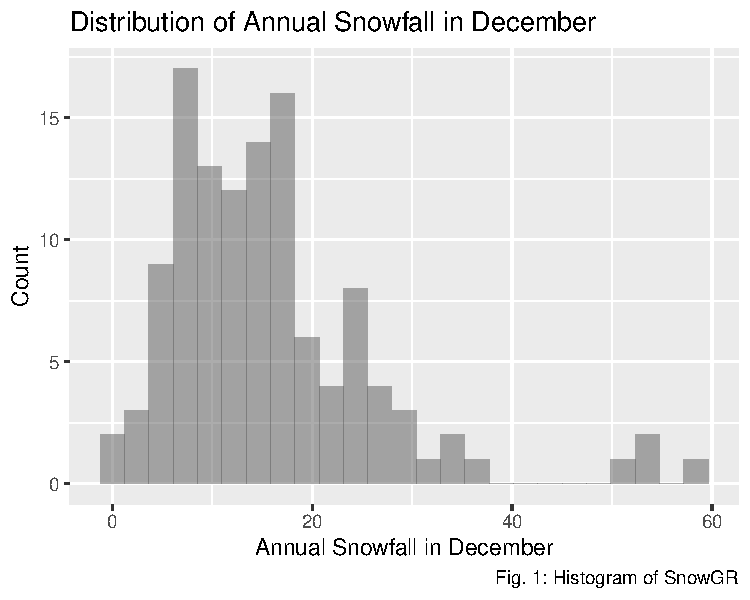
\includegraphics{paper_files/figure-latex/SnowGR histogram-1.pdf} Next,
we will perform the non-parametric bootstrap using 10,000 replications.

\begin{Shaded}
\begin{Highlighting}[]
\FunctionTok{set.seed}\NormalTok{(}\DecValTok{495}\NormalTok{)}
\NormalTok{orig\_mean }\OtherTok{\textless{}{-}} \FunctionTok{mean}\NormalTok{(}\SpecialCharTok{\textasciitilde{}}\NormalTok{ Dec, }\AttributeTok{data =}\NormalTok{ SnowGR) }\CommentTok{\# theta hat}

\FunctionTok{set.seed}\NormalTok{(}\DecValTok{495}\NormalTok{)}
\NormalTok{nboot }\OtherTok{\textless{}{-}} \DecValTok{10000}

\NormalTok{mean }\OtherTok{\textless{}{-}} \FunctionTok{rep}\NormalTok{(}\DecValTok{0}\NormalTok{,nboot)}
\NormalTok{sd }\OtherTok{\textless{}{-}} \FunctionTok{rep}\NormalTok{(}\DecValTok{0}\NormalTok{,nboot)}
\NormalTok{se }\OtherTok{\textless{}{-}} \FunctionTok{rep}\NormalTok{(}\DecValTok{0}\NormalTok{,nboot)}
\NormalTok{t\_stat }\OtherTok{\textless{}{-}} \FunctionTok{rep}\NormalTok{(}\DecValTok{0}\NormalTok{,nboot)}

\ControlFlowTok{for}\NormalTok{ (i }\ControlFlowTok{in} \DecValTok{1}\SpecialCharTok{:}\NormalTok{nboot) \{}
\NormalTok{  resampled }\OtherTok{\textless{}{-}} \FunctionTok{as.data.frame}\NormalTok{(mosaic}\SpecialCharTok{::}\FunctionTok{resample}\NormalTok{(SnowGR, }\AttributeTok{replace =} \ConstantTok{TRUE}\NormalTok{))}
\NormalTok{  mean[i] }\OtherTok{\textless{}{-}} \FunctionTok{mean}\NormalTok{(}\SpecialCharTok{\textasciitilde{}}\NormalTok{Dec, }\AttributeTok{data =}\NormalTok{ resampled)}
\NormalTok{  sd[i] }\OtherTok{\textless{}{-}} \FunctionTok{sd}\NormalTok{(}\SpecialCharTok{\textasciitilde{}}\NormalTok{Dec, }\AttributeTok{data =}\NormalTok{ resampled)}
\NormalTok{\}}

\NormalTok{dec\_means }\OtherTok{\textless{}{-}} \FunctionTok{as.data.frame}\NormalTok{(mean)}
\end{Highlighting}
\end{Shaded}

Figure 2 shows the histogram of bootstrapped values. Since we performed
a large number of bootstrap replications, the bootstrapped distribution
appears to be approximately Normal.

\begin{Shaded}
\begin{Highlighting}[]
\FunctionTok{gf\_dhistogram}\NormalTok{(}\SpecialCharTok{\textasciitilde{}}\NormalTok{ mean, }\AttributeTok{data =}\NormalTok{ dec\_means) }\SpecialCharTok{\%\textgreater{}\%}
  \FunctionTok{gf\_dens}\NormalTok{() }\SpecialCharTok{\%\textgreater{}\%}
  \FunctionTok{gf\_labs}\NormalTok{(}\AttributeTok{title =} \StringTok{"Histogram of 10,000 Bootstrapped Mean Dec Values"}\NormalTok{,}
          \AttributeTok{caption =} \StringTok{"Fig. 2: Bootstrap histogram of Dec values"}\NormalTok{)}
\end{Highlighting}
\end{Shaded}

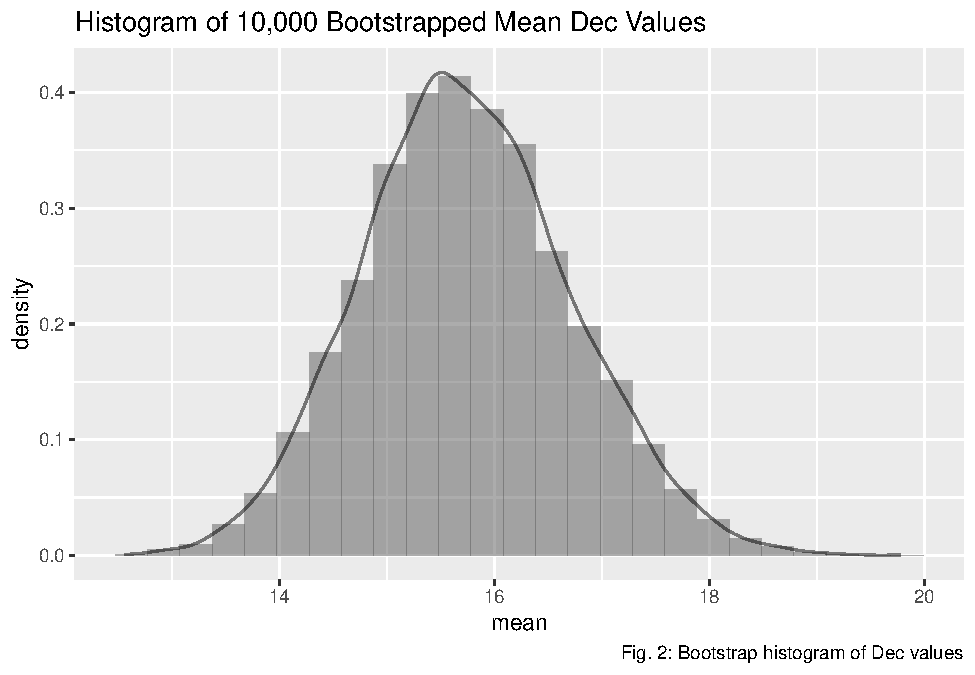
\includegraphics{paper_files/figure-latex/unnamed-chunk-1-1.pdf}

\hypertarget{standard-confidence-interval}{%
\subsection{Standard Confidence
Interval}\label{standard-confidence-interval}}

Confidence intervals are tools that are used to estimate a parameter.
Specifically, a confidence interval gives a range of values in which the
true value of the parameter may lie. An \(\alpha\)-level standard
confidence interval is given by
\[\hat{\theta}_S[\alpha] = \hat{\theta} \pm z_{\alpha}\hat{\sigma},\]
where \(\hat{\theta}\) is a point estimate of the parameter of interest
\(\theta\), \(\hat{\sigma}\) is the estimate of the standard deviation
of \(\hat{\theta}\) and \(z_{\alpha}\) is the \((100 *\alpha)\)th
percentile of the normal deviation \citep{Efron86}. We say that the
confidence interval constructed in this manner can capture the true
parameter with a probability of \(\alpha\).

The standard confidence interval is built based on the assumption that
the distribution we are sampling is Normal. The standard confidence
interval is sometimes called the normal confidence interval for a
bootstrapped sample. This means that the standard confidence interval
could present an incorrect range for an unknown skewed distribution.
However, the same process can be used with bootstrap sampling to form
the bootstrap percentile method. This way, an approximate bootstrap
confidence interval will be created in the same automatic way that the
standard confidence interval was created. For bootstrapped confidence
intervals, the number of bootstrap replications \(B\) must be large
(around 2,000) due to the nature of confidence intervals requiring
greater accuracy \citep{Efron86}.

\hypertarget{standard-confidence-interval-in-use}{%
\subsubsection{Standard Confidence Interval in
Use}\label{standard-confidence-interval-in-use}}

Using our previous example to find a 95\% confidence interval for the
population mean of \texttt{Dec}, we would get the following confidence
interval:

\begin{Shaded}
\begin{Highlighting}[]
\FunctionTok{mean}\NormalTok{(}\SpecialCharTok{\textasciitilde{}}\NormalTok{ Dec, }\AttributeTok{data =}\NormalTok{ SnowGR) }\SpecialCharTok{+} \FunctionTok{qnorm}\NormalTok{(}\FunctionTok{c}\NormalTok{(}\FloatTok{0.025}\NormalTok{, }\FloatTok{0.975}\NormalTok{)) }\SpecialCharTok{*} 
  \FunctionTok{sd}\NormalTok{(}\SpecialCharTok{\textasciitilde{}}\NormalTok{ Dec, }\AttributeTok{data =}\NormalTok{ SnowGR)}\SpecialCharTok{/}\FunctionTok{sqrt}\NormalTok{(}\FunctionTok{nrow}\NormalTok{(SnowGR))}
\end{Highlighting}
\end{Shaded}

\begin{verbatim}
## [1] 13.85639 17.65957
\end{verbatim}

Therefore, we are 95\% confident that the true mean number of inches of
snow that fall in December is between 13.86 inches and 17.66 inches. Our
original histogram with the confidence interval is shown (Figure 3).

\begin{Shaded}
\begin{Highlighting}[]
\FunctionTok{gf\_histogram}\NormalTok{(}\SpecialCharTok{\textasciitilde{}}\NormalTok{ Dec, }\AttributeTok{data =}\NormalTok{ SnowGR) }\SpecialCharTok{+}
  \FunctionTok{labs}\NormalTok{(}\AttributeTok{x =} \StringTok{"Annual Snowfall in December"}\NormalTok{, }
       \AttributeTok{title =} \StringTok{"Distribution of Annual Snowfall in December"}\NormalTok{, }\AttributeTok{y =} \StringTok{"Count"}\NormalTok{,}
       \AttributeTok{caption =} \StringTok{"Fig. 3: Histogram with Standard Interval Shown"}\NormalTok{) }\SpecialCharTok{+}
  \FunctionTok{geom\_vline}\NormalTok{(}\FunctionTok{aes}\NormalTok{(}\AttributeTok{xintercept=} \FloatTok{13.85639}\NormalTok{)) }\SpecialCharTok{+}
  \FunctionTok{geom\_vline}\NormalTok{(}\FunctionTok{aes}\NormalTok{(}\AttributeTok{xintercept=} \FloatTok{17.65957}\NormalTok{))}
\end{Highlighting}
\end{Shaded}

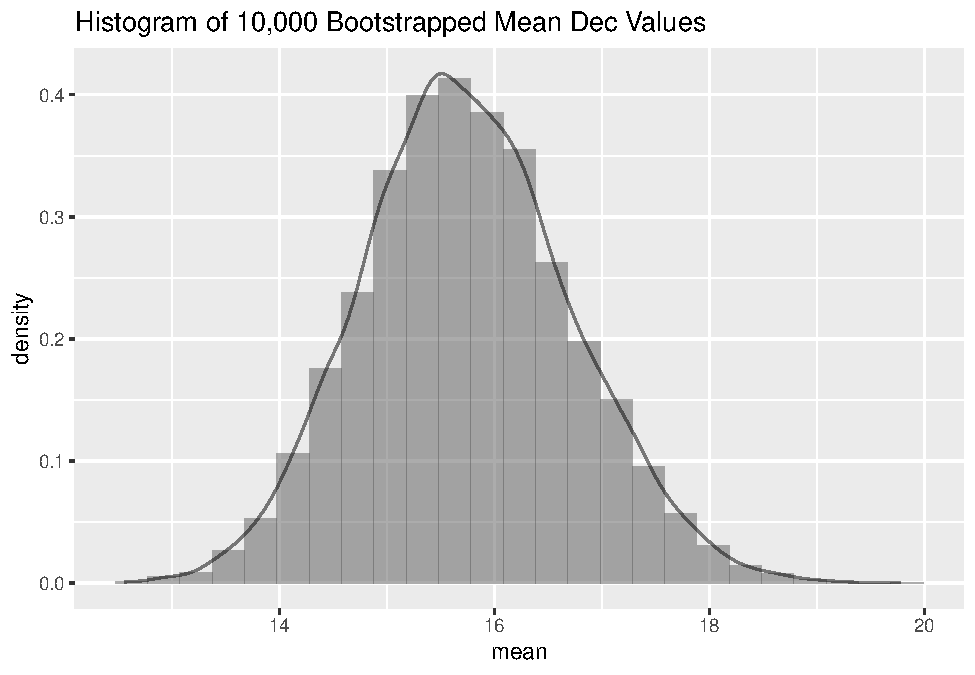
\includegraphics{paper_files/figure-latex/unnamed-chunk-3-1.pdf}

\hypertarget{the-percentile-method}{%
\subsection{The Percentile Method}\label{the-percentile-method}}

The percentile method interval is defined as the interval between the
\(100 * \alpha\) and the \(100(1 - \alpha)\) percentiles of the
bootstrap distribution of \(\hat{\theta}\). That is, the
\((1 - 2\alpha)\) coverage interval can be defined as
\([\hat{\theta}^*_\alpha,\hat{\theta}^*_{1-\alpha}]\)
\citep[\citet{EfronCasi}]{Efron86}. To go further, we can define
\(\hat{G}(t)\) as the bootstrap cdf, or the proportion of bootstrap
samples less than \(t\):
\[\hat{G}(t) = \frac{\#\{\hat{\theta}^{*b} \leq t\}}{B}.\] Thus the
\(\alpha\)th percentile point of the distribution is given by
\[\hat{\theta}_p[\alpha] = \hat{\theta^*_\alpha} = \hat{G}^{-1}(\alpha).\]
It follows that the percentile interval can be represented as
\[\left [ \hat{G}^{-1}(\alpha),\hat{G}^{-1}(1-\alpha) \right ].\] In the
case that the bootstrap distribution of
\(\hat{\theta}^* \sim N(\hat{\theta}, \hat{\sigma}^2)\), the
corresponding percentile interval would be equivalent to the standard
interval. However, this is only sometimes the case. When the bootstrap
distribution is non-normal, we can suppose that there exists, for all
\(\theta\), \[\hat{\phi} \sim N(\phi, \tau^2),\] for some monotone
transformation \(\hat{\phi} = g(\hat{\theta}), \phi = g(\theta)\), and
\(\tau\) is a constant. In other words, this transformation perfectly
normalizes the distribution of \(\hat{\theta}\). This transformation
invariant can be applied to the bootstrap replications such that
\[\hat{\phi}^{*b} = g\left( \hat{\theta}^{*b}\right ) \text{ for } b = 1,2,\dots, B.\]
The corresponding percentiles of the distribution transform similarly,
\(\hat{\phi}^*_\alpha = g \left ( \hat{\theta}^*_\alpha \right )\). Or
we can say that the \((1 - 2\alpha)\) percentile interval is
\(\hat{\phi} \pm \tau z_\alpha\) which can also be represented as
\([\hat{\phi}^*_\alpha,\hat{\phi}^*_{1-\alpha}]\). This means that the
interval on the \(\theta\) scale can be defined as
\[\hat{\theta}^*_\alpha = g^{-1}(\hat{\phi} \pm \tau z_\alpha).\] This
also can be represented as an interval,
\[\left [ g^{-1}(\hat{\phi} \pm \tau z_{1-\alpha}), g^{-1}(\hat{\phi} \pm \tau z_\alpha) \right ].\]
Therefore, the percentile method produces a correct interval for
\(\phi\) and, due to the transformation invariance, also produces a
correct percentile interval for \(\theta\). This method assumes the
existence of some monotone normalizing mapping
\(\hat{\phi} = g(\hat{\theta}), \phi = g(\theta)\) and relies on that to
create a correct interval. Since the process is automatic, we do not
need to know the transformation itself, only that it exists. However, in
some cases, no monotone normalizing mapping will exist \citep{Efron86}.

\hypertarget{the-percentile-method-in-use}{%
\subsubsection{The Percentile Method in
Use}\label{the-percentile-method-in-use}}

Finding a 95\% confidence interval for the true population mean of
\texttt{Dec} using the percentile method, we get:

\begin{Shaded}
\begin{Highlighting}[]
\FunctionTok{qdata}\NormalTok{(}\SpecialCharTok{\textasciitilde{}}\NormalTok{ mean, }\FunctionTok{c}\NormalTok{(}\FloatTok{0.025}\NormalTok{, }\FloatTok{0.975}\NormalTok{), }\AttributeTok{data =}\NormalTok{ dec\_means)}
\end{Highlighting}
\end{Shaded}

\begin{verbatim}
##     2.5%    97.5% 
## 13.91170 17.72353
\end{verbatim}

Therefore, we can say that we are 95\% confident that the true
population mean of inches of snow that fall in December is between 13.91
inches and 17.72 inches. Our original histogram with the percentile
confidence interval is shown (Figure 4).

\begin{Shaded}
\begin{Highlighting}[]
\FunctionTok{gf\_histogram}\NormalTok{(}\SpecialCharTok{\textasciitilde{}}\NormalTok{ Dec, }\AttributeTok{data =}\NormalTok{ SnowGR) }\SpecialCharTok{+}
  \FunctionTok{labs}\NormalTok{(}\AttributeTok{x =} \StringTok{"Annual Snowfall in December"}\NormalTok{, }
       \AttributeTok{title =} \StringTok{"Distribution of Annual Snowfall in December"}\NormalTok{, }\AttributeTok{y =} \StringTok{"Count"}\NormalTok{,}
       \AttributeTok{caption =} \StringTok{"Fig. 4: Histogram with Percentile Interval Shown"}\NormalTok{) }\SpecialCharTok{+}
  \FunctionTok{geom\_vline}\NormalTok{(}\FunctionTok{aes}\NormalTok{(}\AttributeTok{xintercept=} \FloatTok{13.91170}\NormalTok{)) }\SpecialCharTok{+}
  \FunctionTok{geom\_vline}\NormalTok{(}\FunctionTok{aes}\NormalTok{(}\AttributeTok{xintercept=} \FloatTok{17.72353}\NormalTok{))}
\end{Highlighting}
\end{Shaded}

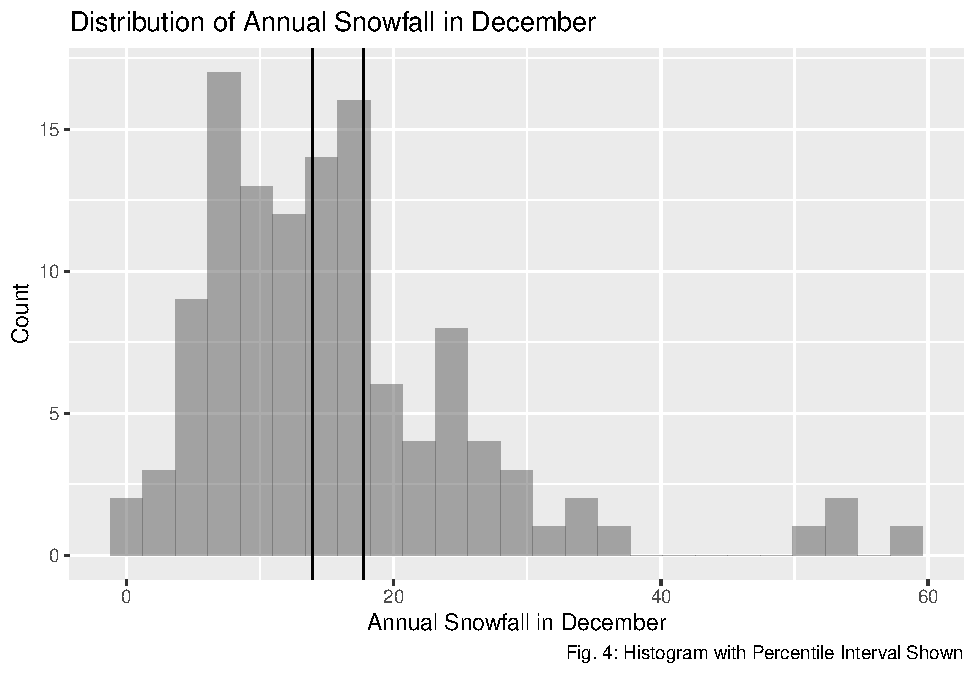
\includegraphics{paper_files/figure-latex/unnamed-chunk-5-1.pdf} This
interval is similar to the one created using the standard method, but
shifted slightly to the right.

\hypertarget{the-bias-corrected-bc-method}{%
\subsection{The Bias-Corrected (BC)
Method}\label{the-bias-corrected-bc-method}}

The following method we will be looking at is the bias-corrected
percentile method (BC method) which is an improvement upon the previous
percentile method because we now consider the possibility of bias. It
can be shown that \(\hat{\theta}\) is biased upwards relative to
\(\theta\), which means that the confidence intervals should be adjusted
downwards \citep[\citet{EfronCasi}]{Efron86}. From our simulated
bootstrap replications
\(\hat{\theta}^{*1}, \hat{\theta}^{*2}, \dots ,\hat{\theta}^{*B},\)
define \[p_0 = \frac{\#\{\hat{\theta}^{*b} \leq \theta\}}{B},\] and
define the bias-correction value \[z_0 = \Phi^{-1}(p_0),\] where
\(\Phi^{-1}\) is the inverse function of the standard normal cdf. Thus,
we define a transformation
\(\hat{\phi} = g(\hat{\theta)}, \phi = g(\theta)\) such that for any
\(\theta\), \[\hat{\phi} \sim N(\phi - z_0\tau, \tau^2),\] with \(z_0\)
and \(\tau\) constants. This means that we can say the bias-corrected
method has an \(\alpha\)-level endpoint which can be represented as
\[\hat{\theta}_{BC}[\alpha] = \hat{G}^{-1} \left [ \Phi \left ( 2z_0 + z_\alpha\right ) \right ].\]
If \(\hat{G} = 0.50\), then half of the bootstrap distribution is less
than \(\hat{\theta}\) and our bias-correction value \(z_0 = 0\). In this
case, the confidence interval produced by BC would be the same interval
that was produced by the percentile method.

\hypertarget{the-bc-method-in-use}{%
\subsubsection{The BC Method in Use}\label{the-bc-method-in-use}}

Using this method to create a 95\% confidence interval has a couple more
steps because we need to find the bias-correction value
\citep{EfronCasi}. First, we calculate the sample mean:

\begin{Shaded}
\begin{Highlighting}[]
\NormalTok{sample\_mean }\OtherTok{\textless{}{-}} \FunctionTok{mean}\NormalTok{(}\SpecialCharTok{\textasciitilde{}}\NormalTok{Dec, }\AttributeTok{data =}\NormalTok{ SnowGR); sample\_mean}
\end{Highlighting}
\end{Shaded}

\begin{verbatim}
## [1] 15.75798
\end{verbatim}

Then we find the proportion of bootstrap replications that have a sample
mean less than the original sample mean.

\begin{Shaded}
\begin{Highlighting}[]
\NormalTok{less\_than\_sample\_mean }\OtherTok{\textless{}{-}} \FunctionTok{sum}\NormalTok{(}\FunctionTok{ifelse}\NormalTok{(dec\_means }\SpecialCharTok{\textless{}=}\NormalTok{ sample\_mean, }\DecValTok{1}\NormalTok{, }\DecValTok{0}\NormalTok{))}\SpecialCharTok{/}\DecValTok{10000}
\NormalTok{less\_than\_sample\_mean}
\end{Highlighting}
\end{Shaded}

\begin{verbatim}
## [1] 0.5208
\end{verbatim}

From this, we can calculate the bias-correction value, \(z_0\):

\begin{Shaded}
\begin{Highlighting}[]
\NormalTok{z0 }\OtherTok{\textless{}{-}} \FunctionTok{qnorm}\NormalTok{(less\_than\_sample\_mean); z0}
\end{Highlighting}
\end{Shaded}

\begin{verbatim}
## [1] 0.05216151
\end{verbatim}

Then we can find the modified percentiles and get the corresponding
confidence interval:

\begin{Shaded}
\begin{Highlighting}[]
\NormalTok{alpha\_lower }\OtherTok{\textless{}{-}} \FloatTok{0.025}\NormalTok{; alpha\_upper }\OtherTok{\textless{}{-}} \FloatTok{0.975}

\NormalTok{new\_lower }\OtherTok{\textless{}{-}} \FunctionTok{pnorm}\NormalTok{(}\DecValTok{2}\SpecialCharTok{*}\NormalTok{z0 }\SpecialCharTok{+} \FunctionTok{qnorm}\NormalTok{(alpha\_lower)); }
\NormalTok{new\_upper }\OtherTok{\textless{}{-}} \FunctionTok{pnorm}\NormalTok{(}\DecValTok{2}\SpecialCharTok{*}\NormalTok{z0 }\SpecialCharTok{+} \FunctionTok{qnorm}\NormalTok{(alpha\_upper)); }

\FunctionTok{qdata}\NormalTok{(}\SpecialCharTok{\textasciitilde{}}\NormalTok{ mean, }\FunctionTok{c}\NormalTok{(new\_lower, new\_upper), }\AttributeTok{data =}\NormalTok{ dec\_means)}
\end{Highlighting}
\end{Shaded}

\begin{verbatim}
## 3.175238% 98.05047% 
##  14.01172  17.82017
\end{verbatim}

Therefore, we are 95\% confident that the true mean inches of snow that
fall in December in Grand Rapids, Michigan is between 14.01 inches and
17.82 inches. Our histogram (Figure 5) is shown.

\begin{Shaded}
\begin{Highlighting}[]
\FunctionTok{gf\_histogram}\NormalTok{(}\SpecialCharTok{\textasciitilde{}}\NormalTok{ Dec, }\AttributeTok{data =}\NormalTok{ SnowGR) }\SpecialCharTok{+}
  \FunctionTok{labs}\NormalTok{(}\AttributeTok{x =} \StringTok{"Annual Snowfall in December"}\NormalTok{, }
       \AttributeTok{title =} \StringTok{"Distribution of Annual Snowfall in December"}\NormalTok{, }\AttributeTok{y =} \StringTok{"Count"}\NormalTok{,}
       \AttributeTok{caption =} \StringTok{"Fig. 5: Histogram with BC Interval Shown"}\NormalTok{) }\SpecialCharTok{+}
  \FunctionTok{geom\_vline}\NormalTok{(}\FunctionTok{aes}\NormalTok{(}\AttributeTok{xintercept=} \FloatTok{14.01172}\NormalTok{)) }\SpecialCharTok{+}
  \FunctionTok{geom\_vline}\NormalTok{(}\FunctionTok{aes}\NormalTok{(}\AttributeTok{xintercept=} \FloatTok{17.82017}\NormalTok{))}
\end{Highlighting}
\end{Shaded}

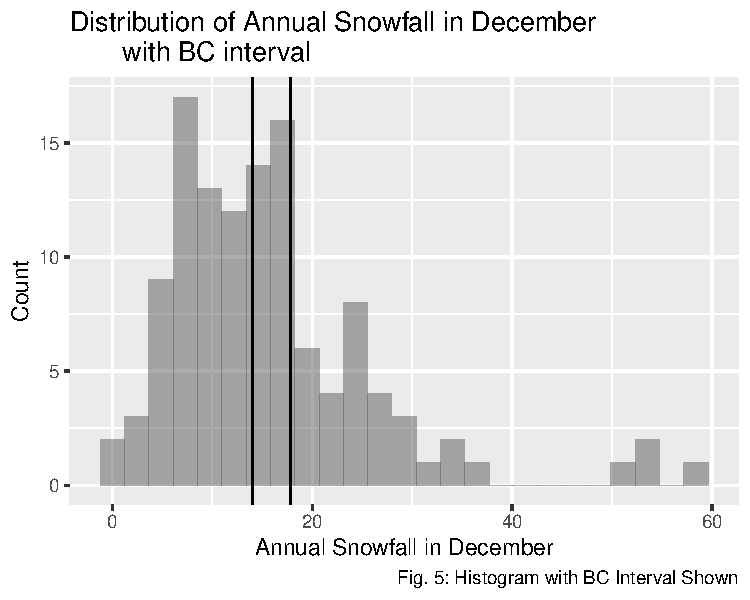
\includegraphics{paper_files/figure-latex/unnamed-chunk-10-1.pdf}

\hypertarget{the-bias-corrected-and-accelerated-bca-method}{%
\subsection{The Bias-Corrected and Accelerated (BCa)
Method}\label{the-bias-corrected-and-accelerated-bca-method}}

The bias-corrected and accelerated method (BCa) further modifies the BC
interval. This method does not assume that the standard error, \(\tau\),
is constant as we did in the BC interval
\citep[\citet{EfronCasi}]{Efron86}. Rather, we assume the existence of a
monotone transformation
\(\hat{\phi} = g(\hat{\theta)}, \phi = g(\theta)\) such that for any
\(\theta\),
\[\hat{\phi} \sim N(\phi - z_0\tau_\phi, \tau_\phi^2) \text{ where } \tau_\phi = 1+ a\phi.\]
The \(a\) is known as the acceleration and is a constant that describes
how the standard deviation of \(\hat{\phi}\) varies with \(\phi\). In
other words, \(a\) is proportional to the skewness of the bootstrap
distribution. For example, \(a=z_0\) for one-parameter exponential
families. However, there are many different algorithms to compute and
estimate \(a\) \citep{Flowers18}. Now, our \(\alpha\)-level endpoint for
a BCa confidence interval is
\[\hat{\theta}_{BCa}[\alpha] = \hat{G}^{-1} \left [ \Phi \left ( z_0 + \frac{z_0+z_\alpha}{1-a(z_0+z_a)} \right ) \right ].\]
We can observe that if \(a = 0\), then
\(\hat{\theta}_{BCa}[\alpha] = \hat{\theta}_{BC}[\alpha].\) When
calculating a BCa confidence interval, the acceleration value, \(a\), is
not a function of the bootstrap distribution and must be calculated
separately. However, the process is algorithmic and can be calculated
without too much work. As we saw, each of the three previous methods
(percentile, BC, and BCa) all build upon each other and have less
restrictive assumptions, but computation increases as we loosen
assumptions.

\hypertarget{the-bca-confidence-interval-in-use}{%
\subsubsection{The BCa Confidence Interval in
Use}\label{the-bca-confidence-interval-in-use}}

In practice, we can use the jackknife procedure to estimate the
acceleration value for this method \citep{EfronCasi}. The jackknife
procedure is a different resampling technique often used to estimate the
bias and variance of a large population. Thus, we will run the jackknife
procedure:

\begin{Shaded}
\begin{Highlighting}[]
\NormalTok{theta }\OtherTok{\textless{}{-}} \ControlFlowTok{function}\NormalTok{(x)\{}\FunctionTok{mean}\NormalTok{(x)\}}
\NormalTok{jackknife\_results }\OtherTok{\textless{}{-}}\NormalTok{ bootstrap}\SpecialCharTok{::}\FunctionTok{jackknife}\NormalTok{(SnowGR}\SpecialCharTok{$}\NormalTok{Dec, theta) }
\end{Highlighting}
\end{Shaded}

We find the mean of the jackknife values below:

\begin{Shaded}
\begin{Highlighting}[]
\NormalTok{jack\_mean }\OtherTok{\textless{}{-}} \FunctionTok{mean}\NormalTok{(}\SpecialCharTok{\textasciitilde{}}\NormalTok{ jackknife\_results}\SpecialCharTok{$}\NormalTok{jack.values); jack\_mean}
\end{Highlighting}
\end{Shaded}

\begin{verbatim}
## [1] 15.75798
\end{verbatim}

Then we can compute an approximation for \(a\).

\begin{Shaded}
\begin{Highlighting}[]
\NormalTok{estimated\_a }\OtherTok{\textless{}{-}}\NormalTok{ (}\DecValTok{1}\SpecialCharTok{/}\DecValTok{6}\NormalTok{)}\SpecialCharTok{*}\FunctionTok{sum}\NormalTok{((jackknife\_results}\SpecialCharTok{$}\NormalTok{jack.values }\SpecialCharTok{{-}}\NormalTok{ jack\_mean)}\SpecialCharTok{\^{}}\DecValTok{3}\NormalTok{)}\SpecialCharTok{/}
\NormalTok{  (}\FunctionTok{sum}\NormalTok{((jackknife\_results}\SpecialCharTok{$}\NormalTok{jack.values }\SpecialCharTok{{-}}\NormalTok{ jack\_mean)}\SpecialCharTok{\^{}}\DecValTok{2}\NormalTok{))}\SpecialCharTok{\^{}}\NormalTok{(}\FloatTok{1.5}\NormalTok{); estimated\_a}
\end{Highlighting}
\end{Shaded}

\begin{verbatim}
## [1] -0.02674911
\end{verbatim}

Now, we can find the adjusted percentiles and the bias-corrected with
acceleration confidence interval.

\begin{Shaded}
\begin{Highlighting}[]
\NormalTok{a\_new\_lower }\OtherTok{\textless{}{-}} \FunctionTok{pnorm}\NormalTok{(z0 }\SpecialCharTok{+}\NormalTok{ (z0 }\SpecialCharTok{+} \FunctionTok{qnorm}\NormalTok{(alpha\_lower))}\SpecialCharTok{/}
\NormalTok{                    (}\DecValTok{1}\SpecialCharTok{{-}}\NormalTok{estimated\_a}\SpecialCharTok{*}\NormalTok{(z0 }\SpecialCharTok{+} \FunctionTok{qnorm}\NormalTok{(alpha\_lower)))); }
\NormalTok{a\_new\_upper }\OtherTok{\textless{}{-}} \FunctionTok{pnorm}\NormalTok{(z0 }\SpecialCharTok{+}\NormalTok{ (z0 }\SpecialCharTok{+} \FunctionTok{qnorm}\NormalTok{(alpha\_upper))}\SpecialCharTok{/}
\NormalTok{                     (}\DecValTok{1}\SpecialCharTok{{-}}\NormalTok{estimated\_a}\SpecialCharTok{*}\NormalTok{(z0 }\SpecialCharTok{+} \FunctionTok{qnorm}\NormalTok{(alpha\_upper)))); }
\FunctionTok{qdata}\NormalTok{(}\SpecialCharTok{\textasciitilde{}}\NormalTok{ mean, }\FunctionTok{c}\NormalTok{(a\_new\_lower, a\_new\_upper), }\AttributeTok{data =}\NormalTok{ dec\_means)}
\end{Highlighting}
\end{Shaded}

\begin{verbatim}
## 2.510119% 97.50908% 
##  13.91591  17.72353
\end{verbatim}

We are 95\% confident that the true mean number of inches of snow that
fall in December is between 13.92 inches and 17.72 inches. Figure 6
shows our confidence interval.

\begin{Shaded}
\begin{Highlighting}[]
\FunctionTok{gf\_histogram}\NormalTok{(}\SpecialCharTok{\textasciitilde{}}\NormalTok{ Dec, }\AttributeTok{data =}\NormalTok{ SnowGR) }\SpecialCharTok{+}
  \FunctionTok{labs}\NormalTok{(}\AttributeTok{x =} \StringTok{"Annual Snowfall in December"}\NormalTok{, }
       \AttributeTok{title =} \StringTok{"Distribution of Annual Snowfall in December"}\NormalTok{, }\AttributeTok{y =} \StringTok{"Count"}\NormalTok{,}
       \AttributeTok{caption =} \StringTok{"Fig. 6: Histogram with BCa Interval Shown"}\NormalTok{) }\SpecialCharTok{+}
  \FunctionTok{geom\_vline}\NormalTok{(}\FunctionTok{aes}\NormalTok{(}\AttributeTok{xintercept=} \FloatTok{13.91591}\NormalTok{)) }\SpecialCharTok{+}
  \FunctionTok{geom\_vline}\NormalTok{(}\FunctionTok{aes}\NormalTok{(}\AttributeTok{xintercept=} \FloatTok{17.72353}\NormalTok{))}
\end{Highlighting}
\end{Shaded}

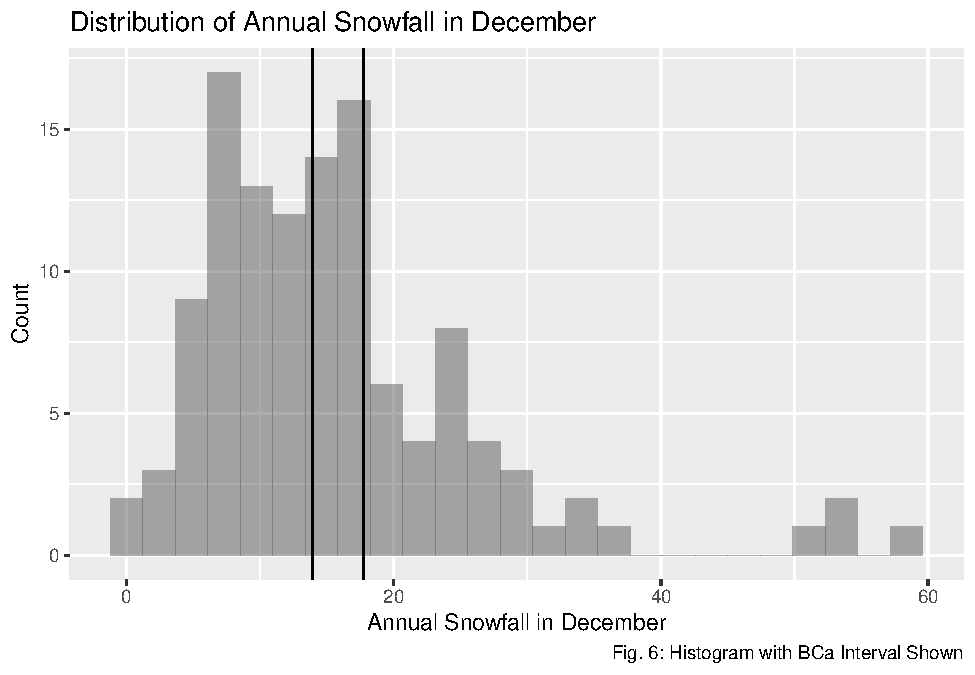
\includegraphics{paper_files/figure-latex/unnamed-chunk-15-1.pdf}

\hypertarget{the-bootstrap-t-studentized-method}{%
\subsection{The Bootstrap-t (Studentized)
Method}\label{the-bootstrap-t-studentized-method}}

The final method we explain is the bootstrap-t interval (or the
studentized method). Recall from earlier, our sample, \(X\) from which
we can calculate an estimate (\(\hat{\theta}(X)\)) of the parameter of
interest \(\theta\) \citep[\citet{Puth15}]{Efron86}. We can also
estimate \(\hat{\sigma}(X)\) for the standard error of \(\theta\). We
can use these parameters to find the Student's \(t\)-statistic defined
as: \[T = \frac{\hat{\theta} - \theta}{\hat{\sigma}}.\] As such, the
\(\alpha\)th percentile point of a confidence interval of \(\theta\)
would be \(\hat{\theta} - \hat{\sigma}T_{(\alpha)}\) where
\(T_{(\alpha)}\) represents the \(\alpha\)th percentile of the
\(t\)-distribution, \(T\). Unfortunately, the percentiles of this
\(t\)-distribution are unknown in most cases, but we can use
bootstrapping to estimate these percentiles. To do this, we perform a
large number, \(B\), of bootstrap samples, from which we can find the
bootstrap replications of the parameter of interest,
\(\hat{\theta^*} = \hat{\theta}(X^*)\), and the standard error,
\(\hat{\sigma^*} = \hat{\sigma}(X^*)\). From these, we can calculate a
t-statistic for each bootstrap sample:
\[T^* = \frac{\hat{\theta}^* - \hat{\theta}}{\hat{\sigma}^*}.\] Using a
large number of these bootstrap samples, we can estimate the percentiles
of the \(t\)-distribution such that:
\[\hat{T}_{(\alpha)} = B*\alpha\text{th ordered value of all the bootstrap replications of }T^*.\]
This means that for \(B = 2,000\) and \(\alpha = 0.90\), then
\(\hat{T}_{(\alpha)}\) is the 1,800th ordered point of all of the
bootstrap replications of \(T^*\). It follows that the \(\alpha\)th
studentized confidence interval endpoint can be given with
\[\hat{\theta}_T[\alpha] = \hat{\theta} - \hat{\sigma}T_{(\alpha)},\]
where we can estimate the standard error using
\[\hat{\sigma} = \frac{1-\hat{\theta}^2}{\sqrt{n}}.\] One of the main
factors why the studentized method is so popular is that we assume that
our bootstrapped statistic is pivotal, which means that the confidence
interval does not depend on any other parameters. Instead, we can
calculate the appropriate confidence interval for the parameter of
interest specifically from the bootstrapped statistics
\citep[\citet{Puth15}]{Efron86}.

\hypertarget{studentized-confidence-interval-in-use}{%
\subsubsection{Studentized Confidence Interval in
Use}\label{studentized-confidence-interval-in-use}}

Following the process above, we can use the following to get our
studentized confidence interval \citep{Lau20}:

\begin{Shaded}
\begin{Highlighting}[]
\FunctionTok{set.seed}\NormalTok{(}\DecValTok{495}\NormalTok{)}
\CommentTok{\# sample statistics}
\NormalTok{orig\_mean }\OtherTok{\textless{}{-}} \FunctionTok{mean}\NormalTok{(}\SpecialCharTok{\textasciitilde{}}\NormalTok{ Dec, }\AttributeTok{data =}\NormalTok{ SnowGR) }\CommentTok{\# theta hat}
\NormalTok{orig\_se }\OtherTok{\textless{}{-}} \FunctionTok{sd}\NormalTok{(}\SpecialCharTok{\textasciitilde{}}\NormalTok{ Dec, }\AttributeTok{data =}\NormalTok{ SnowGR)}\SpecialCharTok{/}\FunctionTok{sqrt}\NormalTok{(}\FunctionTok{nrow}\NormalTok{(SnowGR))}
\CommentTok{\# initialize storage vectors}
\NormalTok{se }\OtherTok{\textless{}{-}} \FunctionTok{rep}\NormalTok{(}\DecValTok{0}\NormalTok{,nboot)}
\NormalTok{t\_stat }\OtherTok{\textless{}{-}} \FunctionTok{rep}\NormalTok{(}\DecValTok{0}\NormalTok{,nboot)}
\CommentTok{\# use bootstrap replication statistics to find se and t{-}stat}
\ControlFlowTok{for}\NormalTok{ (i }\ControlFlowTok{in} \DecValTok{1}\SpecialCharTok{:}\NormalTok{nboot) \{}
\NormalTok{  se[i] }\OtherTok{\textless{}{-}}\NormalTok{ sd[i]}\SpecialCharTok{/}\FunctionTok{sqrt}\NormalTok{(}\FunctionTok{nrow}\NormalTok{(SnowGR))}
\NormalTok{  t\_stat[i] }\OtherTok{\textless{}{-}}\NormalTok{ (mean[i] }\SpecialCharTok{{-}}\NormalTok{ orig\_mean)}\SpecialCharTok{/}\NormalTok{se[i]}
\NormalTok{\}}
\CommentTok{\#find interval}
\NormalTok{dec\_t\_stat }\OtherTok{\textless{}{-}} \FunctionTok{as.data.frame}\NormalTok{(t\_stat)}
\NormalTok{q }\OtherTok{\textless{}{-}} \FunctionTok{unname}\NormalTok{(}\FunctionTok{quantile}\NormalTok{(dec\_t\_stat}\SpecialCharTok{$}\NormalTok{t\_stat, }\FunctionTok{c}\NormalTok{(}\FloatTok{0.025}\NormalTok{, }\FloatTok{0.975}\NormalTok{)))}
\NormalTok{lower }\OtherTok{\textless{}{-}}\NormalTok{ q[}\DecValTok{1}\NormalTok{]}
\NormalTok{upper }\OtherTok{\textless{}{-}}\NormalTok{ q[}\DecValTok{2}\NormalTok{]}
\FunctionTok{c}\NormalTok{(orig\_mean }\SpecialCharTok{{-}}\NormalTok{ upper}\SpecialCharTok{*}\NormalTok{orig\_se, orig\_mean }\SpecialCharTok{{-}}\NormalTok{ lower}\SpecialCharTok{*}\NormalTok{orig\_se)}
\end{Highlighting}
\end{Shaded}

\begin{verbatim}
## [1] 14.03467 18.01709
\end{verbatim}

So we are 95\% confident that the true mean number of inches of snow
that fall in December in Grand Rapids, Michigan is between 14.03 inches
and 18.02 inches. This would give us the following confidence interval
(Figure 7):

\begin{Shaded}
\begin{Highlighting}[]
\FunctionTok{gf\_histogram}\NormalTok{(}\SpecialCharTok{\textasciitilde{}}\NormalTok{ Dec, }\AttributeTok{data =}\NormalTok{ SnowGR) }\SpecialCharTok{+}
  \FunctionTok{labs}\NormalTok{(}\AttributeTok{x =} \StringTok{"Annual Snowfall in December"}\NormalTok{, }
       \AttributeTok{title =} \StringTok{"Distribution of Annual Snowfall in December"}\NormalTok{, }\AttributeTok{y =} \StringTok{"Count"}\NormalTok{, }
       \AttributeTok{caption =} \StringTok{"Fig. 7: Histogram with Studentized Interval Shown"}\NormalTok{) }\SpecialCharTok{+}
  \FunctionTok{geom\_vline}\NormalTok{(}\FunctionTok{aes}\NormalTok{(}\AttributeTok{xintercept=} \FloatTok{14.03467}\NormalTok{)) }\SpecialCharTok{+}
  \FunctionTok{geom\_vline}\NormalTok{(}\FunctionTok{aes}\NormalTok{(}\AttributeTok{xintercept=} \FloatTok{18.01709}\NormalTok{)) }
\end{Highlighting}
\end{Shaded}

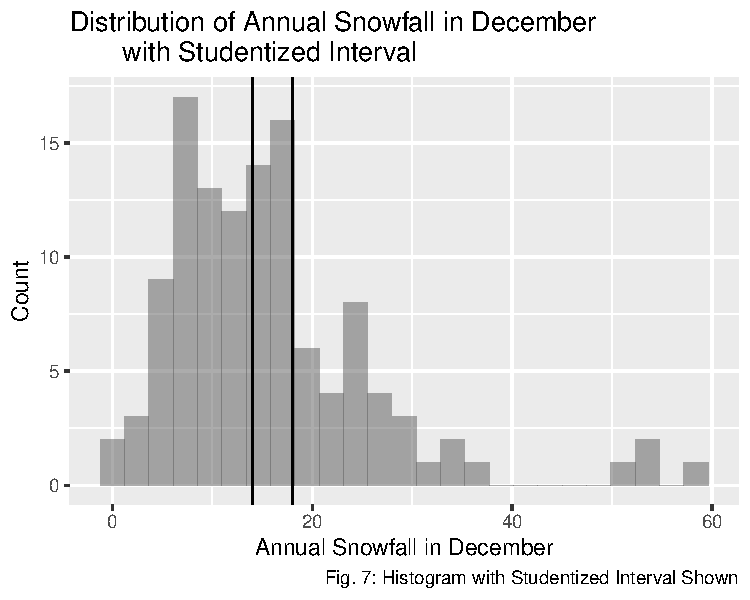
\includegraphics{paper_files/figure-latex/unnamed-chunk-17-1.pdf}

\hypertarget{simulation}{%
\section{Simulation}\label{simulation}}

\hypertarget{code}{%
\subsection{Code}\label{code}}

For our simulation, we will randomly sample from distributions in which
we know the true population mean. For example, we will be sampling from
a Gamma distribution where we can find the true population mean using
the shape and rate parameters of the sample distribution. After we
sample from the distribution, we will create a bootstrapped confidence
interval for a few of the methods we described in the exposition. Since
we know the true population mean of the distribution, we will determine
if the true population mean is contained in the confidence interval for
each of the methods we are testing \citep{Guillaume21}. We will perform
this process a large number of times (10,000 simulations) and then
average by the number of iterations to determine, on average, the
proportion that each bootstrapped confidence interval method contains
the true population mean for a given distribution. We will do this for a
couple of different distributions and ranges of sample sizes to show how
the intervals perform with skewed distributions and larger sample sizes.

To do this simulation, we will use the \texttt{boot} package
\citep{boot}. This package can compute a bootstrap object which contains
the output from a bootstrap calculation of a given sample and then
produces confidence intervals from the bootstrap object. In particular,
we will use the \texttt{boot.ci} function to create four confidence
intervals: the standard (or normal) confidence interval, the studentized
confidence interval, the percentile confidence interval, and the
bias-corrected with acceleration confidence interval.

To start, we will declare some constants, including the sample sizes and
the number of bootstrap replications we use. We will be using a range of
sample sizes from 5 to 150. For this simulation, we will use a
confidence level of 95\%.

\begin{Shaded}
\begin{Highlighting}[]
\NormalTok{sample\_sizes }\OtherTok{\textless{}{-}} \FunctionTok{c}\NormalTok{(}\DecValTok{5}\NormalTok{, }\DecValTok{10}\NormalTok{, }\DecValTok{15}\NormalTok{, }\DecValTok{20}\NormalTok{, }\DecValTok{30}\NormalTok{, }\DecValTok{40}\NormalTok{, }\DecValTok{60}\NormalTok{, }\DecValTok{100}\NormalTok{, }\DecValTok{150}\NormalTok{)}
\NormalTok{num\_sample\_sizes }\OtherTok{\textless{}{-}} \FunctionTok{length}\NormalTok{(sample\_sizes)}
\NormalTok{boot\_reps }\OtherTok{\textless{}{-}} \DecValTok{2000}
\end{Highlighting}
\end{Shaded}

Next, we create a simulation that randomly selects a sample from a
Normal distribution and performs a bootstrap with 2,000 bootstrap
replications. Then, we create the confidence intervals from this
bootstrap and determine if the true mean, our population parameter, is
contained within our intervals. Since we are using a \(Normal(0,1)\)
distribution, our true population mean equals 0. We will repeat this
process 10,000 times as specified for each sample size we are testing.
Since we are initially sampling from a Normal distribution, the
assumptions we hold for the standard interval are true. Thus, we would
expect all of the methods to perform comparably to each other at large
sample sizes.

\begin{Shaded}
\begin{Highlighting}[]
\NormalTok{run\_sim\_normal }\OtherTok{\textless{}{-}} \ControlFlowTok{function}\NormalTok{(sim\_reps) \{}
  \CommentTok{\# create function to return mean and sd of bootstrap replication}
\NormalTok{  boot.stat }\OtherTok{\textless{}{-}} \ControlFlowTok{function}\NormalTok{(d, i) \{}
\NormalTok{    d }\OtherTok{\textless{}{-}}\NormalTok{ X[i]}
    \FunctionTok{return}\NormalTok{ (}\FunctionTok{c}\NormalTok{(}\FunctionTok{mean}\NormalTok{(d), }\FunctionTok{sd}\NormalTok{(d)))}
\NormalTok{  \}}
  \CommentTok{\# initialize matrix to hold different bootstrap prop. for each sample size}
\NormalTok{  master }\OtherTok{\textless{}{-}} \FunctionTok{matrix}\NormalTok{(}\AttributeTok{nrow =}\NormalTok{ num\_sample\_sizes, }\AttributeTok{ncol =} \DecValTok{5}\NormalTok{)}
  \CommentTok{\# iterate through each sample size}
  \ControlFlowTok{for}\NormalTok{(i }\ControlFlowTok{in} \DecValTok{1}\SpecialCharTok{:}\NormalTok{num\_sample\_sizes) \{}
    \CommentTok{\# initialize vectors that hold if the CI contains true mean by iteration}
\NormalTok{    norm\_contains }\OtherTok{\textless{}{-}} \FunctionTok{rep}\NormalTok{(}\DecValTok{0}\NormalTok{, sim\_reps)}
\NormalTok{    student\_contains }\OtherTok{\textless{}{-}} \FunctionTok{rep}\NormalTok{(}\DecValTok{0}\NormalTok{, sim\_reps)}
\NormalTok{    percentile\_contains }\OtherTok{\textless{}{-}} \FunctionTok{rep}\NormalTok{(}\DecValTok{0}\NormalTok{, sim\_reps)}
\NormalTok{    bca\_contains }\OtherTok{\textless{}{-}} \FunctionTok{rep}\NormalTok{(}\DecValTok{0}\NormalTok{, sim\_reps)}
    \CommentTok{\# }
\NormalTok{    n }\OtherTok{\textless{}{-}}\NormalTok{ sample\_sizes[i]}
\NormalTok{    true\_mean }\OtherTok{\textless{}{-}} \DecValTok{0}
    \CommentTok{\# perform 10,000 iterations of bootstraps}
    \ControlFlowTok{for}\NormalTok{ (j }\ControlFlowTok{in} \DecValTok{1}\SpecialCharTok{:}\NormalTok{sim\_reps) \{}
\NormalTok{      X }\OtherTok{\textless{}{-}} \FunctionTok{rnorm}\NormalTok{(n, }\DecValTok{0}\NormalTok{, }\DecValTok{1}\NormalTok{)}
\NormalTok{      values }\OtherTok{\textless{}{-}} \FunctionTok{data.frame}\NormalTok{(X)}
      \CommentTok{\# perform bootstrap and CIs}
\NormalTok{      results }\OtherTok{\textless{}{-}} \FunctionTok{boot}\NormalTok{(}\AttributeTok{data =}\NormalTok{ values, }\AttributeTok{statistic =}\NormalTok{ boot.stat, }\AttributeTok{R =}\NormalTok{ boot\_reps)}
\NormalTok{      ci }\OtherTok{\textless{}{-}} \FunctionTok{boot.ci}\NormalTok{(results, }\AttributeTok{conf =} \FloatTok{0.95}\NormalTok{, }
                    \AttributeTok{type =} \FunctionTok{c}\NormalTok{(}\StringTok{"norm"}\NormalTok{, }\StringTok{"perc"}\NormalTok{, }\StringTok{"bca"}\NormalTok{, }\StringTok{"stud"}\NormalTok{))}
      \CommentTok{\# update vectors depending on if the CI contains true mean}
\NormalTok{      norm\_contains[j] }\OtherTok{\textless{}{-}}\NormalTok{ true\_mean }\SpecialCharTok{\textgreater{}=}\NormalTok{ ci}\SpecialCharTok{$}\NormalTok{normal[}\DecValTok{2}\NormalTok{] }\SpecialCharTok{\&} 
\NormalTok{        true\_mean }\SpecialCharTok{\textless{}=}\NormalTok{ ci}\SpecialCharTok{$}\NormalTok{normal[}\DecValTok{3}\NormalTok{]}
\NormalTok{      student\_contains[j] }\OtherTok{\textless{}{-}}\NormalTok{ true\_mean }\SpecialCharTok{\textgreater{}=}\NormalTok{ ci}\SpecialCharTok{$}\NormalTok{student[}\DecValTok{4}\NormalTok{] }\SpecialCharTok{\&} 
\NormalTok{        true\_mean }\SpecialCharTok{\textless{}=}\NormalTok{ ci}\SpecialCharTok{$}\NormalTok{student[}\DecValTok{5}\NormalTok{]}
\NormalTok{      percentile\_contains[j] }\OtherTok{\textless{}{-}}\NormalTok{ true\_mean }\SpecialCharTok{\textgreater{}=}\NormalTok{ ci}\SpecialCharTok{$}\NormalTok{percent[}\DecValTok{4}\NormalTok{] }\SpecialCharTok{\&} 
\NormalTok{        true\_mean }\SpecialCharTok{\textless{}=}\NormalTok{ ci}\SpecialCharTok{$}\NormalTok{percent[}\DecValTok{5}\NormalTok{]}
\NormalTok{      bca\_contains[j] }\OtherTok{\textless{}{-}}\NormalTok{ true\_mean }\SpecialCharTok{\textgreater{}=}\NormalTok{ ci}\SpecialCharTok{$}\NormalTok{bca[}\DecValTok{4}\NormalTok{] }\SpecialCharTok{\&}
\NormalTok{        true\_mean }\SpecialCharTok{\textless{}=}\NormalTok{ ci}\SpecialCharTok{$}\NormalTok{bca[}\DecValTok{5}\NormalTok{]}
\NormalTok{    \}}
    \CommentTok{\# add the sample size and average proportion to matrix}
\NormalTok{    master[i, }\DecValTok{1}\NormalTok{] }\OtherTok{\textless{}{-}}\NormalTok{ sample\_sizes[i]}
\NormalTok{    master[i, }\DecValTok{2}\NormalTok{] }\OtherTok{\textless{}{-}} \FunctionTok{sum}\NormalTok{(norm\_contains)}\SpecialCharTok{/}\NormalTok{sim\_reps}
\NormalTok{    master[i, }\DecValTok{3}\NormalTok{] }\OtherTok{\textless{}{-}} \FunctionTok{sum}\NormalTok{(student\_contains)}\SpecialCharTok{/}\NormalTok{sim\_reps}
\NormalTok{    master[i, }\DecValTok{4}\NormalTok{] }\OtherTok{\textless{}{-}} \FunctionTok{sum}\NormalTok{(percentile\_contains)}\SpecialCharTok{/}\NormalTok{sim\_reps}
\NormalTok{    master[i, }\DecValTok{5}\NormalTok{] }\OtherTok{\textless{}{-}} \FunctionTok{sum}\NormalTok{(bca\_contains)}\SpecialCharTok{/}\NormalTok{sim\_reps}
\NormalTok{  \}}
  \CommentTok{\# some wrangling}
\NormalTok{  master\_df }\OtherTok{\textless{}{-}} \FunctionTok{as.data.frame}\NormalTok{(master) }\SpecialCharTok{\%\textgreater{}\%} 
      \FunctionTok{rename}\NormalTok{(}\StringTok{"Sample\_Size"} \OtherTok{=}\NormalTok{ V1, }\StringTok{"Normal"} \OtherTok{=}\NormalTok{ V2, }\StringTok{"Studentized"} \OtherTok{=}\NormalTok{ V3, }
             \StringTok{"Percentile"} \OtherTok{=}\NormalTok{ V4, }\StringTok{"BCa"} \OtherTok{=}\NormalTok{ V5) }
\NormalTok{  master\_df}
\NormalTok{\}}
\end{Highlighting}
\end{Shaded}

Secondly, we select from a Gamma Distribution with a shape parameter of
one and a scale parameter of four (\(Gamma(1,4)\)). Therefore, the true
population mean is 4 because the product of the shape and scale
parameters gives the true mean. This simulation follows the same process
as above, where we sampled from the Normal distribution, except we are
sampling from a Gamma distribution this time. Since our Gamma
distribution is heavily left-skewed, we expect the studentized
confidence interval and the BCa confidence interval to perform the best.

\begin{Shaded}
\begin{Highlighting}[]
\NormalTok{run\_sim\_gamma }\OtherTok{\textless{}{-}} \ControlFlowTok{function}\NormalTok{(sim\_reps) \{}
\NormalTok{  boot.stat }\OtherTok{\textless{}{-}} \ControlFlowTok{function}\NormalTok{(d, i) \{}
\NormalTok{    d }\OtherTok{\textless{}{-}}\NormalTok{ X[i]}
    \FunctionTok{return}\NormalTok{ (}\FunctionTok{c}\NormalTok{(}\FunctionTok{mean}\NormalTok{(d), }\FunctionTok{sd}\NormalTok{(d)))}
\NormalTok{  \}}
\NormalTok{  master }\OtherTok{\textless{}{-}} \FunctionTok{matrix}\NormalTok{(}\AttributeTok{nrow =}\NormalTok{ num\_sample\_sizes, }\AttributeTok{ncol =} \DecValTok{5}\NormalTok{)}
  \ControlFlowTok{for}\NormalTok{(i }\ControlFlowTok{in} \DecValTok{1}\SpecialCharTok{:}\NormalTok{num\_sample\_sizes) \{}
\NormalTok{    norm\_contains }\OtherTok{\textless{}{-}} \FunctionTok{rep}\NormalTok{(}\DecValTok{0}\NormalTok{, sim\_reps)}
\NormalTok{    student\_contains }\OtherTok{\textless{}{-}} \FunctionTok{rep}\NormalTok{(}\DecValTok{0}\NormalTok{, sim\_reps)}
\NormalTok{    percentile\_contains }\OtherTok{\textless{}{-}} \FunctionTok{rep}\NormalTok{(}\DecValTok{0}\NormalTok{, sim\_reps)}
\NormalTok{    bca\_contains }\OtherTok{\textless{}{-}} \FunctionTok{rep}\NormalTok{(}\DecValTok{0}\NormalTok{, sim\_reps)}
\NormalTok{    n }\OtherTok{\textless{}{-}}\NormalTok{ sample\_sizes[i]}
\NormalTok{    true\_mean }\OtherTok{\textless{}{-}} \DecValTok{4}
    \ControlFlowTok{for}\NormalTok{ (j }\ControlFlowTok{in} \DecValTok{1}\SpecialCharTok{:}\NormalTok{sim\_reps) \{}
\NormalTok{      X }\OtherTok{\textless{}{-}} \FunctionTok{rgamma}\NormalTok{(sample\_sizes, }\AttributeTok{shape =} \DecValTok{1}\NormalTok{, }\AttributeTok{scale =} \DecValTok{4}\NormalTok{)}
\NormalTok{      values }\OtherTok{\textless{}{-}} \FunctionTok{data.frame}\NormalTok{(X)}
\NormalTok{      results }\OtherTok{\textless{}{-}} \FunctionTok{boot}\NormalTok{(}\AttributeTok{data =}\NormalTok{ values, }\AttributeTok{statistic =}\NormalTok{ boot.stat, }\AttributeTok{R =}\NormalTok{ boot\_reps)}
\NormalTok{      ci }\OtherTok{\textless{}{-}} \FunctionTok{boot.ci}\NormalTok{(results, }\AttributeTok{conf =} \FloatTok{0.95}\NormalTok{, }
                    \AttributeTok{type =} \FunctionTok{c}\NormalTok{(}\StringTok{"norm"}\NormalTok{, }\StringTok{"perc"}\NormalTok{, }\StringTok{"bca"}\NormalTok{, }\StringTok{"stud"}\NormalTok{))}
\NormalTok{      norm\_contains[j] }\OtherTok{\textless{}{-}}\NormalTok{ true\_mean }\SpecialCharTok{\textgreater{}=}\NormalTok{ ci}\SpecialCharTok{$}\NormalTok{normal[}\DecValTok{2}\NormalTok{] }\SpecialCharTok{\&} 
\NormalTok{        true\_mean }\SpecialCharTok{\textless{}=}\NormalTok{ ci}\SpecialCharTok{$}\NormalTok{normal[}\DecValTok{3}\NormalTok{]}
\NormalTok{      student\_contains[j] }\OtherTok{\textless{}{-}}\NormalTok{ true\_mean }\SpecialCharTok{\textgreater{}=}\NormalTok{ ci}\SpecialCharTok{$}\NormalTok{student[}\DecValTok{4}\NormalTok{] }\SpecialCharTok{\&} 
\NormalTok{        true\_mean }\SpecialCharTok{\textless{}=}\NormalTok{ ci}\SpecialCharTok{$}\NormalTok{student[}\DecValTok{5}\NormalTok{]}
\NormalTok{      percentile\_contains[j] }\OtherTok{\textless{}{-}}\NormalTok{ true\_mean }\SpecialCharTok{\textgreater{}=}\NormalTok{ ci}\SpecialCharTok{$}\NormalTok{percent[}\DecValTok{4}\NormalTok{] }\SpecialCharTok{\&} 
\NormalTok{        true\_mean }\SpecialCharTok{\textless{}=}\NormalTok{ ci}\SpecialCharTok{$}\NormalTok{percent[}\DecValTok{5}\NormalTok{]}
\NormalTok{      bca\_contains[j] }\OtherTok{\textless{}{-}}\NormalTok{ true\_mean }\SpecialCharTok{\textgreater{}=}\NormalTok{ ci}\SpecialCharTok{$}\NormalTok{bca[}\DecValTok{4}\NormalTok{] }\SpecialCharTok{\&} 
\NormalTok{        true\_mean }\SpecialCharTok{\textless{}=}\NormalTok{ ci}\SpecialCharTok{$}\NormalTok{bca[}\DecValTok{5}\NormalTok{]}
\NormalTok{    \}}
\NormalTok{    master[i, }\DecValTok{1}\NormalTok{] }\OtherTok{\textless{}{-}}\NormalTok{ sample\_sizes[i]}
\NormalTok{    master[i, }\DecValTok{2}\NormalTok{] }\OtherTok{\textless{}{-}} \FunctionTok{sum}\NormalTok{(norm\_contains)}\SpecialCharTok{/}\NormalTok{sim\_reps}
\NormalTok{    master[i, }\DecValTok{3}\NormalTok{] }\OtherTok{\textless{}{-}} \FunctionTok{sum}\NormalTok{(student\_contains)}\SpecialCharTok{/}\NormalTok{sim\_reps}
\NormalTok{    master[i, }\DecValTok{4}\NormalTok{] }\OtherTok{\textless{}{-}} \FunctionTok{sum}\NormalTok{(percentile\_contains)}\SpecialCharTok{/}\NormalTok{sim\_reps}
\NormalTok{    master[i, }\DecValTok{5}\NormalTok{] }\OtherTok{\textless{}{-}} \FunctionTok{sum}\NormalTok{(bca\_contains)}\SpecialCharTok{/}\NormalTok{sim\_reps}
\NormalTok{  \}}
\NormalTok{  master\_df }\OtherTok{\textless{}{-}} \FunctionTok{as.data.frame}\NormalTok{(master) }\SpecialCharTok{\%\textgreater{}\%} 
      \FunctionTok{rename}\NormalTok{(}\StringTok{"Sample\_Size"} \OtherTok{=}\NormalTok{ V1, }\StringTok{"Normal"} \OtherTok{=}\NormalTok{ V2, }\StringTok{"Studentized"} \OtherTok{=}\NormalTok{ V3, }
             \StringTok{"Percentile"} \OtherTok{=}\NormalTok{ V4, }\StringTok{"BCa"} \OtherTok{=}\NormalTok{ V5) }
\NormalTok{  master\_df}
\NormalTok{\}}
\end{Highlighting}
\end{Shaded}

Lastly, we will be sampling from a Log-Normal distribution. This means
that if we have a random variable, \(X \sim Lognormal\), then the random
variable, \(Y = ln(X) \sim Normal\). Therefore, the distribution is
left-skewed, although not as heavily as the previously used Gamma
distribution. The true mean of this distribution can be found using
\(E(X) = e^{u+\frac{\sigma^2}{2}}\) which means that for a
\(Lognormal(0,1)\) distribution, we expect the population mean to be
\(e^{\frac{1}{2}}\). Again, we expect the studentized confidence
interval and the BCa confidence interval to perform the best.

\begin{Shaded}
\begin{Highlighting}[]
\NormalTok{run\_sim\_log\_normal }\OtherTok{\textless{}{-}} \ControlFlowTok{function}\NormalTok{(sim\_reps) \{}
\NormalTok{  boot.stat }\OtherTok{\textless{}{-}} \ControlFlowTok{function}\NormalTok{(d, i) \{}
\NormalTok{    d }\OtherTok{\textless{}{-}}\NormalTok{ X[i]}
    \FunctionTok{return}\NormalTok{ (}\FunctionTok{c}\NormalTok{(}\FunctionTok{mean}\NormalTok{(d), }\FunctionTok{sd}\NormalTok{(d)))}
\NormalTok{  \}}
\NormalTok{  master }\OtherTok{\textless{}{-}} \FunctionTok{matrix}\NormalTok{(}\AttributeTok{nrow =}\NormalTok{ num\_sample\_sizes, }\AttributeTok{ncol =} \DecValTok{5}\NormalTok{)}
  \ControlFlowTok{for}\NormalTok{(i }\ControlFlowTok{in} \DecValTok{1}\SpecialCharTok{:}\NormalTok{num\_sample\_sizes) \{}
\NormalTok{    norm\_contains }\OtherTok{\textless{}{-}} \FunctionTok{rep}\NormalTok{(}\DecValTok{0}\NormalTok{, sim\_reps)}
\NormalTok{    student\_contains }\OtherTok{\textless{}{-}} \FunctionTok{rep}\NormalTok{(}\DecValTok{0}\NormalTok{, sim\_reps)}
\NormalTok{    percentile\_contains }\OtherTok{\textless{}{-}} \FunctionTok{rep}\NormalTok{(}\DecValTok{0}\NormalTok{, sim\_reps)}
\NormalTok{    bca\_contains }\OtherTok{\textless{}{-}} \FunctionTok{rep}\NormalTok{(}\DecValTok{0}\NormalTok{, sim\_reps)}
\NormalTok{    n }\OtherTok{\textless{}{-}}\NormalTok{ sample\_sizes[i]}
\NormalTok{    true\_mean }\OtherTok{\textless{}{-}} \FunctionTok{exp}\NormalTok{(}\DecValTok{1}\SpecialCharTok{/}\DecValTok{2}\NormalTok{)}
    \ControlFlowTok{for}\NormalTok{ (j }\ControlFlowTok{in} \DecValTok{1}\SpecialCharTok{:}\NormalTok{sim\_reps) \{}
\NormalTok{      X }\OtherTok{\textless{}{-}} \FunctionTok{rlnorm}\NormalTok{(n, }\DecValTok{0}\NormalTok{, }\DecValTok{1}\NormalTok{)}
\NormalTok{      values }\OtherTok{\textless{}{-}} \FunctionTok{data.frame}\NormalTok{(X)}
\NormalTok{      results }\OtherTok{\textless{}{-}} \FunctionTok{boot}\NormalTok{(}\AttributeTok{data =}\NormalTok{ values, }\AttributeTok{statistic =}\NormalTok{ boot.stat, }\AttributeTok{R =}\NormalTok{ boot\_reps)}
\NormalTok{      ci }\OtherTok{\textless{}{-}} \FunctionTok{boot.ci}\NormalTok{(results, }\AttributeTok{conf =} \FloatTok{0.95}\NormalTok{, }
                    \AttributeTok{type =} \FunctionTok{c}\NormalTok{(}\StringTok{"norm"}\NormalTok{, }\StringTok{"perc"}\NormalTok{, }\StringTok{"bca"}\NormalTok{, }\StringTok{"stud"}\NormalTok{))}
\NormalTok{      norm\_contains[j] }\OtherTok{\textless{}{-}}\NormalTok{ true\_mean }\SpecialCharTok{\textgreater{}=}\NormalTok{ ci}\SpecialCharTok{$}\NormalTok{normal[}\DecValTok{2}\NormalTok{] }\SpecialCharTok{\&} 
\NormalTok{        true\_mean }\SpecialCharTok{\textless{}=}\NormalTok{ ci}\SpecialCharTok{$}\NormalTok{normal[}\DecValTok{3}\NormalTok{]}
\NormalTok{      student\_contains[j] }\OtherTok{\textless{}{-}}\NormalTok{ true\_mean }\SpecialCharTok{\textgreater{}=}\NormalTok{ ci}\SpecialCharTok{$}\NormalTok{student[}\DecValTok{4}\NormalTok{] }\SpecialCharTok{\&} 
\NormalTok{        true\_mean }\SpecialCharTok{\textless{}=}\NormalTok{ ci}\SpecialCharTok{$}\NormalTok{student[}\DecValTok{5}\NormalTok{]}
\NormalTok{      percentile\_contains[j] }\OtherTok{\textless{}{-}}\NormalTok{ true\_mean }\SpecialCharTok{\textgreater{}=}\NormalTok{ ci}\SpecialCharTok{$}\NormalTok{percent[}\DecValTok{4}\NormalTok{] }\SpecialCharTok{\&} 
\NormalTok{        true\_mean }\SpecialCharTok{\textless{}=}\NormalTok{ ci}\SpecialCharTok{$}\NormalTok{percent[}\DecValTok{5}\NormalTok{]}
\NormalTok{      bca\_contains[j] }\OtherTok{\textless{}{-}}\NormalTok{ true\_mean }\SpecialCharTok{\textgreater{}=}\NormalTok{ ci}\SpecialCharTok{$}\NormalTok{bca[}\DecValTok{4}\NormalTok{] }\SpecialCharTok{\&} 
\NormalTok{        true\_mean }\SpecialCharTok{\textless{}=}\NormalTok{ ci}\SpecialCharTok{$}\NormalTok{bca[}\DecValTok{5}\NormalTok{]}
\NormalTok{    \}}
\NormalTok{    master[i, }\DecValTok{1}\NormalTok{] }\OtherTok{\textless{}{-}}\NormalTok{ sample\_sizes[i]}
\NormalTok{    master[i, }\DecValTok{2}\NormalTok{] }\OtherTok{\textless{}{-}} \FunctionTok{sum}\NormalTok{(norm\_contains)}\SpecialCharTok{/}\NormalTok{sim\_reps}
\NormalTok{    master[i, }\DecValTok{3}\NormalTok{] }\OtherTok{\textless{}{-}} \FunctionTok{sum}\NormalTok{(student\_contains)}\SpecialCharTok{/}\NormalTok{sim\_reps}
\NormalTok{    master[i, }\DecValTok{4}\NormalTok{] }\OtherTok{\textless{}{-}} \FunctionTok{sum}\NormalTok{(percentile\_contains)}\SpecialCharTok{/}\NormalTok{sim\_reps}
\NormalTok{    master[i, }\DecValTok{5}\NormalTok{] }\OtherTok{\textless{}{-}} \FunctionTok{sum}\NormalTok{(bca\_contains)}\SpecialCharTok{/}\NormalTok{sim\_reps}
\NormalTok{  \}}
\NormalTok{  master\_df }\OtherTok{\textless{}{-}} \FunctionTok{as.data.frame}\NormalTok{(master) }\SpecialCharTok{\%\textgreater{}\%} 
      \FunctionTok{rename}\NormalTok{(}\StringTok{"Sample\_Size"} \OtherTok{=}\NormalTok{ V1, }\StringTok{"Normal"} \OtherTok{=}\NormalTok{ V2, }\StringTok{"Studentized"} \OtherTok{=}\NormalTok{ V3, }
             \StringTok{"Percentile"} \OtherTok{=}\NormalTok{ V4, }\StringTok{"BCa"} \OtherTok{=}\NormalTok{ V5) }
\NormalTok{  master\_df}
\NormalTok{\}}
\end{Highlighting}
\end{Shaded}

Once we have all the simulations, we can run them below.

\begin{Shaded}
\begin{Highlighting}[]
\FunctionTok{set.seed}\NormalTok{(}\DecValTok{495}\NormalTok{)}
\NormalTok{normal\_df }\OtherTok{\textless{}{-}} \FunctionTok{run\_sim\_normal}\NormalTok{(}\DecValTok{10000}\NormalTok{)}
\FunctionTok{write.csv}\NormalTok{(normal\_df,}\StringTok{"data/normal\_data\_df.csv"}\NormalTok{, }\AttributeTok{row.names =} \ConstantTok{FALSE}\NormalTok{)}

\NormalTok{log\_normal\_df }\OtherTok{\textless{}{-}} \FunctionTok{run\_sim\_log\_normal}\NormalTok{(}\DecValTok{10000}\NormalTok{)}
\FunctionTok{write.csv}\NormalTok{(log\_normal\_df,}\StringTok{"data/log\_normal\_df.csv"}\NormalTok{, }\AttributeTok{row.names =} \ConstantTok{FALSE}\NormalTok{)}

\NormalTok{gamma\_df }\OtherTok{\textless{}{-}} \FunctionTok{run\_sim\_gamma}\NormalTok{(}\DecValTok{10000}\NormalTok{)}
\FunctionTok{write.csv}\NormalTok{(gamma\_df,}\StringTok{"data/gamma\_data\_df.csv"}\NormalTok{, }\AttributeTok{row.names =} \ConstantTok{FALSE}\NormalTok{)}
\end{Highlighting}
\end{Shaded}

After, we can create the graphs and output for each of the distributions
and sample sizes.

\begin{Shaded}
\begin{Highlighting}[]
\NormalTok{normal\_df }\OtherTok{\textless{}{-}} \FunctionTok{read.csv}\NormalTok{(}\AttributeTok{file =} \StringTok{\textquotesingle{}data/normal\_data\_df.csv\textquotesingle{}}\NormalTok{)}
\NormalTok{gamma\_df }\OtherTok{\textless{}{-}} \FunctionTok{read.csv}\NormalTok{(}\AttributeTok{file =} \StringTok{\textquotesingle{}data/gamma\_data\_df.csv\textquotesingle{}}\NormalTok{)}
\NormalTok{log\_normal\_df }\OtherTok{\textless{}{-}} \FunctionTok{read.csv}\NormalTok{(}\AttributeTok{file =} \StringTok{\textquotesingle{}data/log\_normal\_df.csv\textquotesingle{}}\NormalTok{)}

\CommentTok{\# create the figure that shows the normal output }
\NormalTok{normal\_df\_long }\OtherTok{\textless{}{-}}\NormalTok{ normal\_df }\SpecialCharTok{\%\textgreater{}\%}
  \FunctionTok{pivot\_longer}\NormalTok{(}\AttributeTok{cols =} \DecValTok{2}\SpecialCharTok{:}\DecValTok{5}\NormalTok{, }\AttributeTok{names\_to =} \StringTok{"method"}\NormalTok{, }\AttributeTok{values\_to =} \StringTok{"prop"}\NormalTok{) }
    
\NormalTok{normal\_fig }\OtherTok{\textless{}{-}} \FunctionTok{ggplot}\NormalTok{(}\AttributeTok{data =}\NormalTok{ normal\_df\_long, }
                    \FunctionTok{aes}\NormalTok{(}\AttributeTok{x =}\NormalTok{ Sample\_Size, }\AttributeTok{y =}\NormalTok{ prop, }\AttributeTok{color =}\NormalTok{ method)) }\SpecialCharTok{+} 
  \FunctionTok{geom\_point}\NormalTok{() }\SpecialCharTok{+} \FunctionTok{geom\_line}\NormalTok{() }\SpecialCharTok{+} 
  \FunctionTok{labs}\NormalTok{(}
    \AttributeTok{title =} \StringTok{"Prop. of CIs that Contain the True Mean from Normal Distibution"}\NormalTok{, }
    \AttributeTok{x =} \StringTok{"Sample Size"}\NormalTok{, }
    \AttributeTok{y =} \StringTok{"Proportion (of 10,000 Simulations)"}\NormalTok{, }\AttributeTok{color =} \StringTok{"Method"}\NormalTok{,}
    \AttributeTok{caption =} \StringTok{"Fig. 8: Graph showing the Accuracy of Bootstrap CI Methods for}
\StringTok{       different sample sizes on Normal Dist."}\NormalTok{) }\SpecialCharTok{+}
  \FunctionTok{theme\_light}\NormalTok{() }\SpecialCharTok{+}
  \FunctionTok{theme}\NormalTok{(}\AttributeTok{legend.position=}\StringTok{"bottom"}\NormalTok{)}

\CommentTok{\# create the table for the normal output}
\NormalTok{normal\_table }\OtherTok{\textless{}{-}}\NormalTok{ normal\_df }\SpecialCharTok{\%\textgreater{}\%}
  \FunctionTok{kable}\NormalTok{(}\AttributeTok{booktabs =} \ConstantTok{TRUE}\NormalTok{, }\AttributeTok{align =} \StringTok{"c"}\NormalTok{, }
        \AttributeTok{caption =} \StringTok{"From a Normal distribution"}\NormalTok{, }
        \AttributeTok{col.names =} \FunctionTok{gsub}\NormalTok{(}\StringTok{"[\_]"}\NormalTok{, }\StringTok{" "}\NormalTok{, }\FunctionTok{names}\NormalTok{(normal\_df)), }\AttributeTok{digits =} \DecValTok{3}\NormalTok{)}

\CommentTok{\# create the figure that shows the gamma output}
\NormalTok{gamma\_df\_long }\OtherTok{\textless{}{-}}\NormalTok{ gamma\_df }\SpecialCharTok{\%\textgreater{}\%}
  \FunctionTok{pivot\_longer}\NormalTok{(}\AttributeTok{cols =} \DecValTok{2}\SpecialCharTok{:}\DecValTok{5}\NormalTok{, }\AttributeTok{names\_to =} \StringTok{"method"}\NormalTok{, }\AttributeTok{values\_to =} \StringTok{"prop"}\NormalTok{) }
    
\NormalTok{gamma\_fig }\OtherTok{\textless{}{-}} \FunctionTok{ggplot}\NormalTok{(}\AttributeTok{data =}\NormalTok{ gamma\_df\_long, }
                    \FunctionTok{aes}\NormalTok{(}\AttributeTok{x =}\NormalTok{ Sample\_Size, }\AttributeTok{y =}\NormalTok{ prop, }\AttributeTok{color =}\NormalTok{ method)) }\SpecialCharTok{+} 
  \FunctionTok{geom\_point}\NormalTok{() }\SpecialCharTok{+} \FunctionTok{geom\_line}\NormalTok{() }\SpecialCharTok{+} 
  \FunctionTok{labs}\NormalTok{(}\AttributeTok{title =} \StringTok{"Prop. of CIs that Contain the True Mean from Gamma Distibution"}\NormalTok{, }
       \AttributeTok{x =} \StringTok{"Sample Size"}\NormalTok{, }
       \AttributeTok{y =} \StringTok{"Proportion (of 10,000 Simulations)"}\NormalTok{, }\AttributeTok{color =} \StringTok{"Method"}\NormalTok{,}
       \AttributeTok{caption =} \StringTok{"Fig. 9: Graph showing the Accuracy of Bootstrap CI Methods for }
\StringTok{       different sample sizes on Gamma Dist."}\NormalTok{) }\SpecialCharTok{+}
  \FunctionTok{theme\_light}\NormalTok{() }\SpecialCharTok{+}
  \FunctionTok{theme}\NormalTok{(}\AttributeTok{legend.position=}\StringTok{"bottom"}\NormalTok{)}

\CommentTok{\# create the table for the gamma output}
\NormalTok{gamma\_table }\OtherTok{\textless{}{-}}\NormalTok{ gamma\_df }\SpecialCharTok{\%\textgreater{}\%}
  \FunctionTok{kable}\NormalTok{(}\AttributeTok{booktabs =} \ConstantTok{TRUE}\NormalTok{, }\AttributeTok{align =} \StringTok{"c"}\NormalTok{, }
        \AttributeTok{caption =} \StringTok{"From a Gamma distribution"}\NormalTok{, }
        \AttributeTok{col.names =} \FunctionTok{gsub}\NormalTok{(}\StringTok{"[\_]"}\NormalTok{, }\StringTok{" "}\NormalTok{, }\FunctionTok{names}\NormalTok{(gamma\_df)), }\AttributeTok{digits =} \DecValTok{3}\NormalTok{) }
   
\CommentTok{\# create the figure that shows the log normal output}
\NormalTok{log\_normal\_df\_long }\OtherTok{\textless{}{-}}\NormalTok{ log\_normal\_df }\SpecialCharTok{\%\textgreater{}\%}
  \FunctionTok{pivot\_longer}\NormalTok{(}\AttributeTok{cols =} \DecValTok{2}\SpecialCharTok{:}\DecValTok{5}\NormalTok{, }\AttributeTok{names\_to =} \StringTok{"method"}\NormalTok{, }\AttributeTok{values\_to =} \StringTok{"prop"}\NormalTok{) }
    
\NormalTok{log\_normal\_fig }\OtherTok{\textless{}{-}} \FunctionTok{ggplot}\NormalTok{(}\AttributeTok{data =}\NormalTok{ log\_normal\_df\_long, }
                    \FunctionTok{aes}\NormalTok{(}\AttributeTok{x =}\NormalTok{ Sample\_Size, }\AttributeTok{y =}\NormalTok{ prop, }\AttributeTok{color =}\NormalTok{ method)) }\SpecialCharTok{+} 
  \FunctionTok{geom\_point}\NormalTok{() }\SpecialCharTok{+} \FunctionTok{geom\_line}\NormalTok{() }\SpecialCharTok{+} 
  \FunctionTok{labs}\NormalTok{(}\AttributeTok{title =}\StringTok{"Prop. of CIs that Contain True Mean from Log{-}Normal Distibution"}\NormalTok{,}
       \AttributeTok{x =} \StringTok{"Sample Size"}\NormalTok{, }
       \AttributeTok{y =} \StringTok{"Proportion (of 10,000 Simulations)"}\NormalTok{, }\AttributeTok{color =} \StringTok{"Method"}\NormalTok{,}
       \AttributeTok{caption =} \StringTok{"Fig. 10: Graph showing the Accuracy of Bootstrap CI Methods }
\StringTok{       for different sample sizes on Log{-}Normal Dist."}\NormalTok{) }\SpecialCharTok{+}
  \FunctionTok{theme\_light}\NormalTok{() }\SpecialCharTok{+}
  \FunctionTok{theme}\NormalTok{(}\AttributeTok{legend.position=}\StringTok{"bottom"}\NormalTok{)}

\CommentTok{\# create the table for the log normal output}
\NormalTok{log\_normal\_table }\OtherTok{\textless{}{-}}\NormalTok{ log\_normal\_df }\SpecialCharTok{\%\textgreater{}\%}
  \FunctionTok{kable}\NormalTok{(}\AttributeTok{booktabs =} \ConstantTok{TRUE}\NormalTok{, }\AttributeTok{align =} \StringTok{"c"}\NormalTok{, }
        \AttributeTok{caption =} \StringTok{"From a Log{-}Normal distribution"}\NormalTok{, }
        \AttributeTok{col.names =} \FunctionTok{gsub}\NormalTok{(}\StringTok{"[\_]"}\NormalTok{, }\StringTok{" "}\NormalTok{, }\FunctionTok{names}\NormalTok{(log\_normal\_df)), }\AttributeTok{digits =} \DecValTok{3}\NormalTok{)}
\end{Highlighting}
\end{Shaded}

\hypertarget{results}{%
\subsection{Results}\label{results}}

\hypertarget{normal-distribution-simulation}{%
\subsubsection{Normal Distribution
Simulation}\label{normal-distribution-simulation}}

First, we have the results of the simulation where we randomly sampled
from a Normal distribution.

\begin{Shaded}
\begin{Highlighting}[]
\NormalTok{normal\_fig}
\end{Highlighting}
\end{Shaded}

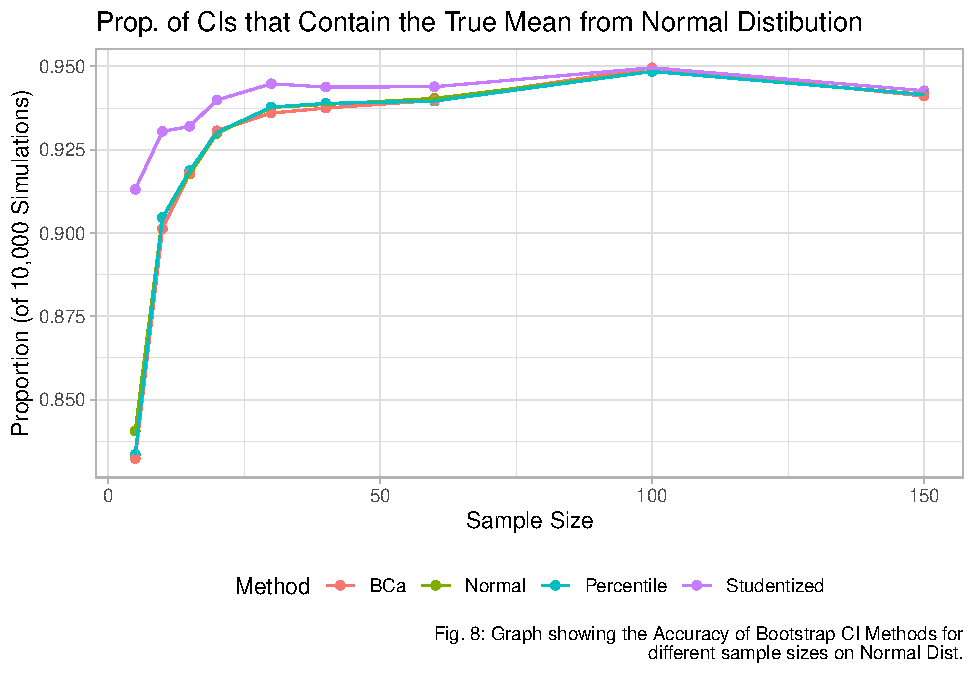
\includegraphics{paper_files/figure-latex/unnamed-chunk-18-1.pdf}

At small sample sizes, the studentized confidence interval performed
much better than the other intervals, which all performed similarly. For
a sample size of 5, the studentized interval had an accuracy of around
91.3\%. In comparison, the other three intervals had an accuracy of
around 83\% to 84\% of creating an interval that contained the true
population mean. The standard, percentile, and BCa confidence interval
methods all have similar processes, especially when the distribution we
are sampling from is Normal because the assumptions we made for the
standard interval are correct. As the sample size increases, the
performance of the intervals increases and rises to stay consistent at
around 94\% to 95\% accuracy. The data (Table 1) is shown for reference.

\begin{Shaded}
\begin{Highlighting}[]
\NormalTok{normal\_table}
\end{Highlighting}
\end{Shaded}

\begin{table}

\caption{\label{tab:create graphs}From a Normal distribution}
\centering
\begin{tabular}[t]{ccccc}
\toprule
Sample Size & Normal & Studentized & Percentile & BCa\\
\midrule
5 & 0.841 & 0.913 & 0.834 & 0.832\\
10 & 0.905 & 0.930 & 0.905 & 0.901\\
15 & 0.918 & 0.932 & 0.919 & 0.918\\
20 & 0.930 & 0.940 & 0.930 & 0.931\\
30 & 0.938 & 0.945 & 0.938 & 0.936\\
\addlinespace
40 & 0.939 & 0.944 & 0.939 & 0.938\\
60 & 0.940 & 0.944 & 0.940 & 0.940\\
100 & 0.949 & 0.950 & 0.949 & 0.950\\
150 & 0.942 & 0.943 & 0.942 & 0.941\\
\bottomrule
\end{tabular}
\end{table}

\hypertarget{gamma-distribution-simulation}{%
\subsubsection{Gamma Distribution
Simulation}\label{gamma-distribution-simulation}}

Second, we have the results from the simulation where we sampled from a
Gamma distribution.

\begin{Shaded}
\begin{Highlighting}[]
\NormalTok{gamma\_fig}
\end{Highlighting}
\end{Shaded}

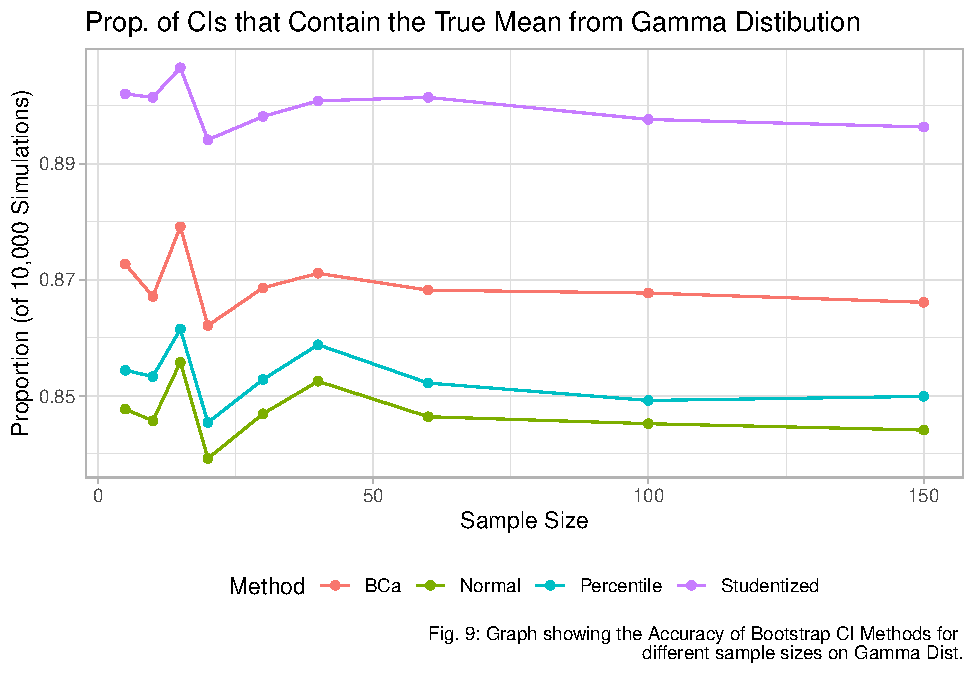
\includegraphics{paper_files/figure-latex/unnamed-chunk-20-1.pdf}

The \(Gamma(1,4)\) distribution we randomly sampled from is
heavily-skewed, so we did not expect all of the bootstrap confidence
interval methods to work comparably. As shown in Figure 9, the
studentized method performed the best at around 90\% accuracy for
creating a confidence interval that contained the true mean. The BCa
method performed the second best at around 87\% accuracy. The percentile
method performed the following best with around 85\% accuracy, while the
standard method performed the worst with an accuracy of around 84.5\%.
As the sample size increased, the accuracy of each of the methods became
less variable and evened out to a constant accuracy. The table
containing the proportions (Table 2) is shown for reference.

\begin{Shaded}
\begin{Highlighting}[]
\NormalTok{gamma\_table}
\end{Highlighting}
\end{Shaded}

\begin{table}

\caption{\label{tab:create graphs}From a Gamma distribution}
\centering
\begin{tabular}[t]{ccccc}
\toprule
Sample Size & Normal & Studentized & Percentile & BCa\\
\midrule
5 & 0.848 & 0.902 & 0.854 & 0.873\\
10 & 0.846 & 0.901 & 0.853 & 0.867\\
15 & 0.856 & 0.906 & 0.862 & 0.879\\
20 & 0.839 & 0.894 & 0.845 & 0.862\\
30 & 0.847 & 0.898 & 0.853 & 0.869\\
\addlinespace
40 & 0.853 & 0.901 & 0.859 & 0.871\\
60 & 0.846 & 0.901 & 0.852 & 0.868\\
100 & 0.845 & 0.898 & 0.849 & 0.868\\
150 & 0.844 & 0.896 & 0.850 & 0.866\\
\bottomrule
\end{tabular}
\end{table}

\hypertarget{log-normal-distribution-simulation}{%
\subsubsection{Log-Normal Distribution
Simulation}\label{log-normal-distribution-simulation}}

Lastly, we have the results from the simulation where we sampled from a
Log-Normal distribution.

\begin{Shaded}
\begin{Highlighting}[]
\NormalTok{log\_normal\_fig}
\end{Highlighting}
\end{Shaded}

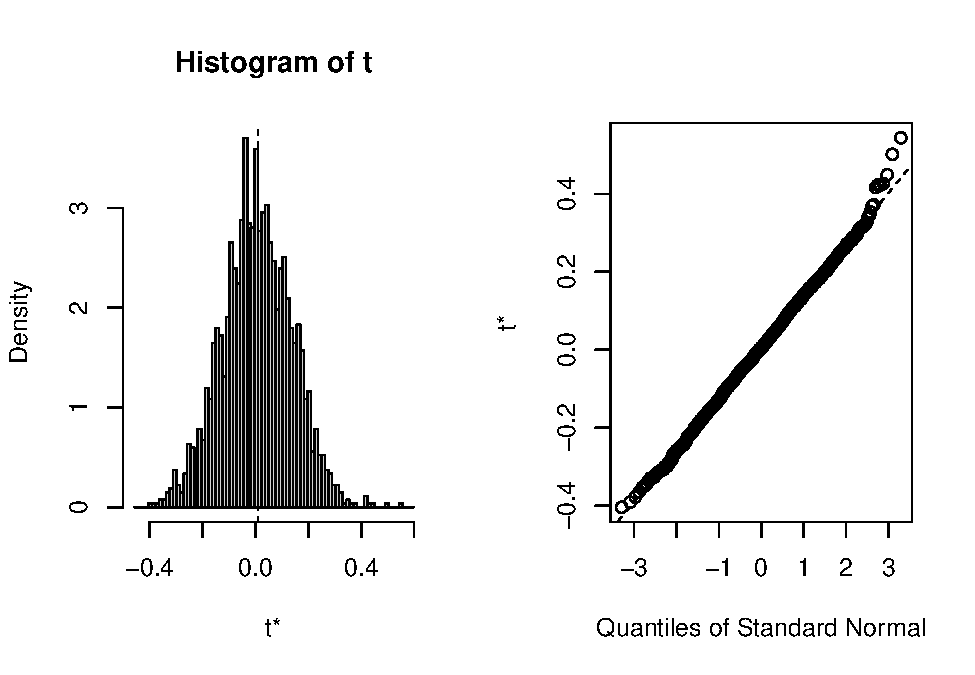
\includegraphics{paper_files/figure-latex/unnamed-chunk-22-1.pdf}

As shown in Figure 10, the studentized method had the greatest accuracy
in creating the confidence intervals that captured the true mean. At
small sample sizes such as 5, the studentized method has an accuracy of
82.3\%, while the following best is the BCa method with a 73.4\%
accuracy. As the sample size increases, all methods' accuracy increases
quickly and performs comparably, although the studentized and BCa
methods perform slightly better. All the intervals stay constant at
around 92.5\% to 93.5\% accuracy for large sample sizes. Again, the
proportions are shown (Table 3) for each sample size for reference.

\begin{Shaded}
\begin{Highlighting}[]
\NormalTok{log\_normal\_table}
\end{Highlighting}
\end{Shaded}

\begin{table}

\caption{\label{tab:create graphs}From a Log-Normal distribution}
\centering
\begin{tabular}[t]{ccccc}
\toprule
Sample Size & Normal & Studentized & Percentile & BCa\\
\midrule
5 & 0.715 & 0.823 & 0.720 & 0.734\\
10 & 0.795 & 0.855 & 0.806 & 0.828\\
15 & 0.829 & 0.876 & 0.839 & 0.862\\
20 & 0.847 & 0.885 & 0.856 & 0.874\\
30 & 0.869 & 0.901 & 0.879 & 0.893\\
\addlinespace
40 & 0.884 & 0.907 & 0.890 & 0.903\\
60 & 0.901 & 0.921 & 0.911 & 0.920\\
100 & 0.912 & 0.926 & 0.917 & 0.919\\
150 & 0.925 & 0.935 & 0.928 & 0.927\\
\bottomrule
\end{tabular}
\end{table}
\newpage

\hypertarget{conclusion}{%
\section{Conclusion}\label{conclusion}}

In this paper, we demonstrated the power of using bootstrapped
confidence intervals to estimate a true population parameter without
using any information about the underlying distribution of the sample.
In the exposition, we introduced the standard method, which relies on
three conditions: 1) that the distribution is Normal, 2) that there is
no bias, and 3) that there is a constant standard error. If we take away
the first condition and use the bootstrap percentiles to create the
interval, we are left with the percentile method. If we add a
bias-correcting value not equal to zero, then we have the
bias-correcting method. Furthermore, if we allow for a non-constant
standard error (through the acceleration), we have the bias-corrected
with acceleration method. Using the studentized method, we can also use
bootstrap resampling to estimate a \(t\)-distribution from which we can
create a confidence interval. From our simulation, the methods all
performed reasonably the same for the Normal distribution at large
sample sizes. However, when we introduced skew into the distributions,
the studentized and BCa methods performed better than the others at
large sample sizes. It is important to note that even at large sample
sizes, none of our methods reached a coverage of 95\%, which was our
specified confidence level. The closest we were was when we sampled from
a Normal distribution. This may be because our sample sizes need to be
bigger; however, we can reach a close approximation using the largest
sample size we tested. Thanks to the high computational power available,
we can use bootstrapping to create confidence intervals for a population
parameter without knowing much about the actual sample.

\bibliographystyle{agsm}
\bibliography{bibliography.bib}


\end{document}
